%%%%%%%%%%%%%%%%%%%%%%%%%%%%%%%%%%%%%%%%%
% University Assignment Title Page
% LaTeX Template
% Version 1.0 (27/12/12)
%
% This template has been downloaded from:
% http://www.LaTeXTemplates.com
%
% Original author:
% WikiBooks (http://en.wikibooks.org/wiki/LaTeX/Title_Creation)
%
% License:
% CC BY-NC-SA 3.0 (http://creativecommons.org/licenses/by-nc-sa/3.0/)
%
% Modified for COSC480/490 by:
% Lech Szymanski (8/3/18)

\documentclass[12pt]{article}
\usepackage[draft]{cosc4x0style}
\usepackage[ruled, linesnumbered,lined]{algorithm2e}
\usepackage{amsmath}
\usepackage{amssymb}
\usepackage{amsthm}
\usepackage{booktabs}
\usepackage{breakcites}
\usepackage{color}
\usepackage{caption}
\usepackage[linguistics]{forest}
\usepackage{longtable}
\usepackage{marginnote}
\usepackage{todonotes}
\usepackage{subcaption}
\usepackage{rotating}
\usepackage{url}

% Custom theorem environment stuff %
% Gets rid of italics
% \theoremstyle{definition}
\newtheoremstyle{grammarstyle}% name
  {10pt}%Space above
  {10pt}%Space below
  {\normalfont}%Body font
  {\parindent}%Indent amount
  {\bfseries}% Theorem head font
  {:}%Punctuation after theorem head
  {\parindent}%Space after theorem head 2
  {}%Theorem head spec (can be left empty, meaning ‘normal’)
\theoremstyle{grammarstyle}

\newtheorem{gram}{Grammar}
% \numberwithin{align}{gram}

% Replace the trailing period with a colon
% \usepackage{xpatch}
% \makeatletter
% \xpatchcmd{\@thm}{\thm@headpunct{.}}{\thm@headpunct{}}{}{}
% \makeatother

% Get rid of parantheses around optional argument
\makeatletter
\def\thmhead@plain#1#2#3{%
  \thmname{#1}\thmnumber{\@ifnotempty{#1}{ }\@upn{#2}}%
  \thmnote{ {\the\thm@notefont#3}}}
\let\thmhead\thmhead@plain
\makeatother

% Code listings styles %
\usepackage{listings}
\usepackage{xcolor}

\definecolor{codegreen}{rgb}{0,0.6,0}
\definecolor{codegray}{rgb}{0.5,0.5,0.5}
\definecolor{codepurple}{rgb}{0.58,0,0.82}

\lstdefinestyle{mystyle}{
    commentstyle=\color{codegreen},
    keywordstyle=\color{magenta},
    numberstyle=\tiny\color{codegray},
    stringstyle=\color{codepurple},
    basicstyle=\ttfamily\footnotesize,
breakatwhitespace=false,
breaklines=true,
captionpos=b,
keepspaces=true,
numbers=left,
numbersep=5pt,
showspaces=false,
    showstringspaces=false,
showtabs=false,
    tabsize=2
}

\lstset{style=mystyle}

\newcommand{\keyword}[1]{%
    \textbf{#1}%
    % Add keyword to the margin
    % \todo[color=none, linecolor=none]{#1}%
}

\usepackage[round]{natbib}   % omit 'round' option if you prefer square brackets
\bibliographystyle{plainnat}
% \bibliographystyle{apalike}
% \usepackage[usenames,dvipsnames,svgnames,table]{xcolor}

% To compile the final version of the report (which will remove all the todo content)
%\usepackage{cosc4x0style}

% Specify project code 480 or 490
\papercode{480}

% Your project title
\title{Quantifying Conceptual Density in Text}

% Your name
\author{Anthony \textsc{Dickson}}
\studentid{3348967}

% Names of your supervisors, separated by line break '\\'
\supervisors{
  Anthony \textsc{Robins} \\
  Alistair \textsc{Knott}
}

% Date, change the \today to a set date if you want to be precise
\reportdate{\today}

\begin{document}
\maketitle

\tableofcontents
\clearpage

\begin{abstract}
    ``Conceptual density'' is a term that describes the degree to which concepts in a domain are integrated, or interdependent.
    There is a hypothesis that text documents with high conceptual density are harder to process.
    At present, the concept of ``conceptual density'' has been informally defined.
    In this pilot study, I investigate the idea of conceptual density in the context of expository text documents, a graph-based model for quantifying conceptual density and ways to evaluate this model. Finally, I discuss open problems and direction for future work related to conceptual density.
    % Talk about why measuring conceptual density would be useful?
\end{abstract}

% \tableofcontents
% \clearpage

\section{Introduction}
\cite{robins2010learning} suggested that a domain of ``tightly integrated concepts'' magnifies the effect of early success or failure of learning, leading to polarised learning outcomes, an effect that he named ``learning edge momentum''. A tightly integrated concept is said to be a concept that is difficult to describe or explain independently of other concepts. This pilot study is focused on the idea of ``conceptual density'', an idea related to the degree to which concepts in a given domain are integrated.

% It is thought that the unusually high rate of fail and high grades observed in introductory programming courses is possibly due to concepts in programming languages being unusually tightly integrated \citep{robins2010learning}.  Robins suggested that a domain of tightly integrated concepts magnifies the effect of early success or failure of learning, leading to polarised learning outcomes, an effect he named learning edge momentum. This report is interested in conceptual density, an idea related to the degree to which concepts in a given domain are integrated.

The idea of conceptual density affecting the difficulty of learning is not unique to the aforementioned work. Cognitive load theory provides a framework for reasoning about aspects of learning difficulty and can be used to guide instructional design \citep{sweller1994cognitive}. Conceptual density appears in the literature on cognitive load theory, in a perhaps slightly different form, as ``element interactivity''. Element interactivity, similar to conceptual density, is an idea related to the number of interacting elements in a task or piece of material that is to be learned. Under the element interactivity effect, high element interactivity is suggested to be the main contributor to the difficulty of a learning task.

To the best of my knowledge, there exists no objective measure in the current literature of the element interactivity effect or the notion of conceptual density. Element interactivity appears to be estimated manually and it depends greatly on the knowledge of the learner \citep{chandler1996cognitive}, and as such remains subjective. In \citep{robins2010learning} the notion of concepts being tightly integrated stems from the observation that educators typically fail to reach a consensus on how to structure introductory programming courses (this is supposedly not the case in many other disciplines). While no measure of conceptual density was clearly defined in that work, some possible ways to do so were proposed.

In this pilot study, I set out to elaborate on the definition of conceptual density and develop an objective measure of this concept in the context of well-structured expository text documents (e.g. textbooks). For measuring conceptual density, I explore one of the methods mentioned in \citep{robins2010learning} - analysing a mind-map like graph structure. Whereas in the original work, this approach was suggested as a characterisation of introductory programming course material that is to be generated by experts, in this pilot study I aim to create a tool that builds up and analyses mind-map like graph structures from a text document automatically, through the use of natural language processing methods and graph analysis techniques, thus removing the need for an expert.

The main contributions of the work in this pilot study are:
(i) the exploration of the notion of conceptual density (Sections \ref{sec:background} and \ref{sec:conceptual_density_in_text});
(ii) a graph-based model for quantifying conceptual density (Sections \ref{sec:conceptual_density_in_text}, \ref{sec:building_a_graph_of_concepts} and \ref{sec:implementation_of_the_conceptual_density_model});
(iii) a framework for quantitatively evaluating the quality of the model (Section \ref{sec:evaluation});
and (iv) a discussion of open problems and direction for future work related to conceptual density
% (Sections
% % \ref{sec:open_problems},
% \ref{sec:related_work}
% and \ref{sec:future_work}).
(Section \ref{sec:future_work}).

% The rest of this report is structured as follows.
% Section \ref{sec:background} covers the theoretical background of conceptual density;
% Section \ref{sec:conceptual_density_in_text} defines what is considered as a concept in text and other text features that relate to conceptual density;
% Section \ref{sec:building_a_graph_of_concepts} describes the parsing algorithm used for building a mind-map like graph structure and how a numerical score of conceptual density can be derived from a graph structure;
% Section \ref{sec:implementation_of_the_conceptual_density_model} describes the implementation of the conceptual density model used in the experiments;
% Section \ref{sec:evaluation} describes methods used for evaluating the quality of the text parsing algorithm and the graph-based model of conceptual density;
% Section \ref{sec:open_problems} discusses open problems relating to conceptual density;
% Section \ref{sec:related_work} discusses related work and what distinguishes the work in this pilot study from the related work;
% and Section \ref{sec:future_work} discusses the work-to-date and future work.

\section{Background} \label{sec:background}
\subsection{Learning Edge Momentum}
\cite{robins2010learning} proposed learning edge momentum as an explanation for the unusually high rate of both fail and high grades in introductory programming courses. The hypothesis builds upon the idea that we learn at the edges of what we know, or in other words, it is easy to learn things that build upon pre-existing knowledge. The core of the hypothesis is that learning outcomes are self-reinforcing: successful learning of a concept tends to make learning closely related concepts easier, and unsuccessful learning tends to make learning closely related concepts more difficult. It is also suggested that concepts in programming languages tend to be tightly integrated and that these tightly integrated concepts are difficult to describe or understand independently of each other. This means that learning a new concept is greatly dependent on understanding the prerequisite concepts. And because of this, the effects of learning edge momentum in introductory programming courses are particularly pronounced, leading to the polarised distribution of grades.

Conceptual density is mentioned in this paper as a possible metric for providing more concrete evidence to educators on how to structure introductory programming courses. Two methods are suggested for measuring the degree to which concepts in a domain are integrated. One method is to look at the proximity of key concept terms and see if there are areas where many concepts are mentioned close together. The other method is to generate a mind-map like graph structure. In this approach, a domain of concepts is represented as a graph structure, where the concepts present in the material are represented with a node in the graph and edges between nodes represent a connection between concepts. This follows the main ideas behind semantic networks and knowledge graphs \citep{sowa1987semantic, zhang2002knowledge, koncel2019text}, which are graph structures used for knowledge representation. This idea of a mind map of concepts forms the basis for the work in this pilot study.

\subsection{Cognitive Load Theory and Schema}
CLT (cognitive load theory) provides a framework for reasoning about learning difficulty and instructional design \citep{sweller1994cognitive}. In CLT the main task of the brain is characterised as information processing, and each person has a certain amount of working memory to process information. Performing tasks requires an amount of mental exertion and concentration, called cognitive load. When the amount of cognitive load exceeds the capacity of an individual's working memory, performing the given task becomes much more difficult.

If we are to explain this by analogy, the idea of working memory is similar in some ways to computer RAM and running out of working memory is akin to what happens when a computer runs out of RAM. When a computer runs out of RAM, it starts thrashing and all of the programs will become very slow and take many times longer to run compared to when there is enough RAM. By reducing the number of programs that are running we can reduce the memory usage and prevent the computer from thrashing. Similarly, under CLT we can reduce cognitive load by reducing the number of things that must be considered simultaneously to perform a given task in order to make it easier to perform that task.

The main contributor to the difficulty of a task is the number of things that must be considered simultaneously and the degree to which they interact. In CLT this idea is captured by \keyword{element interactivity} and the element interactivity effect \citep{sweller2011element}. The cognitive load imposed by element interactivity is said to be intrinsic to the material itself (\keyword{intrinsic cognitive load}), meaning that no matter how you present the material there will be a minimum level of difficulty.

How we present material can affect how difficult it is to understand it. For example, consider trying to teach beginner programmers what all the keywords mean in a Java program that prints ``Hello, World'' to the screen (see Figure \ref{fig:java_hello_world}) and what each part of the code does. This would likely be too much to learn at once. Here there are many interacting elements (e.g. access modifiers, classes, types, functions, function arguments, comments, member fields, member functions, function calls, string literals) just in the code of this simple program. Compare this to pointing out the line that prints the message and the fact that anything between the quotation marks is printed to the terminal window. This approach is much easier to understand since there are fewer things that must be considered. Changing how the material is presented has the effect of increasing or reducing \keyword{extraneous cognitive load}, a type of cognitive load that is not intrinsic to the material itself but dependent on how the material is presented.

\begin{figure}
    \centering
     \lstset{xleftmargin=20pt}
    \lstinputlisting[language=Java]{docs/HelloWorld.java}
    \caption{Example Java program that prints the message ``Hello, World''.}
    \label{fig:java_hello_world}
\end{figure}

Following on with the example, the details of the ``Hello, world'' program could be taught more easily once the learner has learned the fundamentals and acquired a basic intuition for programming. It is theorised that this is because as complex ideas and tasks are learned, we learn more compact representations of these that are committed to long-term memory. These compact representations are often referred to as \keyword{schema}; a schema is essentially a single unit of knowledge representing a concept or task \citep{axelrod1973schema, abelson1981psychological, bartlett1995remembering}. By acquiring a schema, a task with many interacting elements can be reduced to a task with a few elements, or even a single element. And under the element interactivity effect, fewer interacting elements means less overall cognitive load.

To summarise CLT in a rather simplified manner, an individual has a limited amount of working memory to process information and if the amount of cognitive load exceeds the capacity of this working memory, then processing the information becomes much more difficult. There are three things from CLT that we are interested in: element interactivity, which is the main contributor to both intrinsic cognitive load and overall cognitive load; intrinsic cognitive load which is related to the inherent complexity of information; and extraneous load which is influenced by how the material/task is presented.

\section{Conceptual Density in Text} \label{sec:conceptual_density_in_text}
To reiterate, conceptual density is an idea related to the degree to which concepts in a domain are integrated, and in this pilot study, we are interested in conceptual density in the context of text documents. Some questions that we are interested in are, for example: how are concepts related, to what degree are concepts integrated, do concepts form self-referential systems, how are concepts referenced and presented in the document? Conceptual density can be rooted in element interactivity and described in terms of intrinsic cognitive load, and the way that concepts are presented in a document (e.g. how concepts are referenced between sections) can be described in terms of extraneous cognitive load. In this section, I will give a simple working definition of a concept in text and describe a few text features related to the idea of conceptual density.

\subsection{Identifying Concepts in Text} \label{sec:idenifying_concepts}
To understand the relationships between concepts, we must first be able to identify concepts in text. A definition of a concept that could be used is a noun phrase - a phrase in text that denotes a thing. Using words from the previous sentence as an example, both ``definition'' and ``simple definition'' would be valid noun phrases; if we include determiners into the definition of a noun phrase ``a simple definition'' would also be a valid noun phrase. A more precise definition this type of noun phrase is: an optional determiner, followed by a (possibly empty) sequence of nouns and/or adjectives, terminated by a noun. This kind of noun phrase can also be expressed in regex-like syntax using part of speech tags:
\begin{gram}[NP] \label{gr:np_pattern}
\texttt{<DT>?<NN.*|JJ>*<NN.*>}
\end{gram}
\noindent
where the angle brackets denote a group/part of speech tag, \texttt{DT} is a determiner (e.g. a, the), \texttt{NN.*} is any type of noun and \texttt{JJ} is an adjective.

This pattern describes noun phrases such as `apple', `an apple' and `a red apple'. However, these noun phrases may also be joined together by prepositions (e.g. `in' or `of') or coordinating conjunctions (e.g. `and' or `or') to form a single, complex concept. For example, consider the sentence ``Zeus is the sky and thunder god of the ancient Greek religion''. We can see that `the sky and thunder god' is one concept because we are not saying that Zeus is `the sky' and that he is separately the `thunder god', so we have a case for considering two noun phrases joined by a coordinating conjunction as a single concept. It is also evident that we should consider `the sky and thunder god of the ancient Greek religion' as a single, complex concept because Zeus is not the sky and thunder god of all religions, but rather of the ancient Greek religion alone.
I call these types of noun phrases `complex noun phrases'. For this pilot study, I define a concept to be a complex noun phrase, which is a noun phrase optionally followed by a sequence of preposition/coordinating conjunction and noun phrase pairs. We can define a complex noun phrase more precisely as:
\begin{gram}[CNP] \label{gr:cnp_pattern}
    \texttt{<NP>(<IN|CC><NP>)*}
\end{gram}
\noindent
where \texttt{NP} is Grammar \ref{gr:np_pattern}, \texttt{IN} is a preposition and \texttt{CC} is a coordinating conjunction.

\subsection{Presentation of Concepts} \label{sec:presentation of concepts}
The presentation of concepts is the way that concepts are talked about in a document and how concepts are referenced between sections of the document. For example, a concept in section A may require a reference to a concept in section B; likewise a concept in section C may require a reference to a concept in section B. These types of interactions between concepts are of interest, and are of relevance to the idea of conceptual density, since the interaction introduces another element that must be considered simultaneously by the reader.
This increases element interactivity which is the core of cognitive load.
In this section, I will propose two types of concepts present in text, and two types of references that could be used to help measure the effect of presentation on conceptual density.

\subsubsection{A Priori and Emerging Concepts}
It is possible to categorise concepts into two types: a priori and emerging.
An a priori concept is a concept that the reader of a text document would be expected to know beforehand or to be common knowledge.
An emerging concept is a concept that is defined or introduced within a document.
For example, a textbook on computer programming would expect the reader to know what a computer is, but possibly not the concept of recursion. In this case, the concept `computer' would be an a priori concept and `recursion' would be an emerging concept.
The importance of distinguishing between these two types of concepts is in how they contribute to cognitive load differently. Referencing an a priori concept would impose minimal cognitive load since the a priori concept would likely represent a fully acquired schema and well-integrated knowledge. On the other hand, an emerging concept would likely impose more cognitive load since it likely represents a schema that is yet to be fully acquired and still requires a noticeable amount of mental exertion in regards to the concept and its constituent parts.

\subsubsection{Forward References}
Forward references are where the text refers to a concept that is not fully explained until later in the document. These types of references introduce extraneous cognitive load since they make the reader \textit{park} the involved concepts, without much existing knowledge to associate them with. Remembering unfamiliar terms that carry little meaning (to the reader) is more of a demanding task than remembering well-integrated knowledge. For example, when teaching Java programming to beginners the meaning and function of keywords such as \texttt{class} and \texttt{static} are often not explained and are usually just rote learned until later in the course.

\subsubsection{Backward References}
Backward references are where the text refers to a concept that was explained previously in the text. These types of references are likely to be introducing a relation between concepts. The cost of backward references is relatively low when compared to forward references. With forward references, we are making the readers consider an additional element that is not at all well understood by the reader, along with the current context. However, in the case of backward references, we are asking the reader to recall a previously explained concept and possibly introduce a new relationship between the two concepts. This type of reference imposes less cognitive load as it allows the reader to call on pre-existing knowledge.

\section{Building a Graph of Concepts} \label{sec:building_a_graph_of_concepts}
The domain of concepts present in a text document can be represented with a graph structure. The graph structure that is being built is similar to a mind-map, except instead of a single central idea/concept, we are building a rather free-form graph with concepts branching off other related concepts. Representing a domain of concepts in this type of graph has precedent in semantic networks/knowledge graphs.
% This graph-based approach is a natural approach for the problem of quantifying conceptual density because the core concern is the degree to which concepts are integrated, in other words the relationships between the concepts. With respect to the quantification of conceptual density, well-established graph theory and related analysis techniques provide ways to derive a numerical score of conceptual density.
In this section, I will describe how we can build a graph of concepts from text, and how we can extract concepts and the text features described in the previous section.

\subsection{Nodes and Extracting Concepts}
In the graph structure we are building, a node represents a concept present in a given text document. As discussed in Section \ref{sec:idenifying_concepts}, we create a definition of what constitutes a concept in terms of patterns of parts of speech. The formal definition of the pattern given defines what is called a grammar. The basic process to extract a concept from text is to segment the document into sentences, then split each sentence into a set of tokens (words separated by white-space), then for each set of tokens we assign a tag to each token denoting the part of speech of the token. From here we chunk the sentences into groupings based on the patterns described in the grammars. An example is shown in Figure \ref{fig:parse_tree_example}.


\begin{figure}[t]
    \centering
    \makebox[\textwidth][c]{
        \begin{forest}
        for tree={
            if n children=0{
              tier=terminal,
            }{},
        }
        [S
        [CNP
        [NP
                    [NN[Bread]]
                ]
        ]
        [VBZ [is]]
            [VBN[prepared]]
            [IN[from]]
        [CNP
        [NP
                    [DT[a]]
                    [NN[dough]]
        ]
                [IN[of]]
                [NP
                    [NN[wheat]]
                    [NN[flour]]
                ]
                [CC[and]]
        [NP
                    [NN[water]]
                ]
            ]
        ]
        \end{forest}
    }
    \caption{The parse tree resulting from first tagging the parts of speech for tokens in the sentence ``Bread is prepared from a dough of wheat flour and water'', and then chunking the tagged tokens using the regex grammars defined in Grammar \ref{gr:np_pattern} and Grammar \ref{gr:cnp_pattern}. The nodes directly above the terminal nodes denote each word's part of speech tag. The tag `S' represents a sentence, the tag `VBZ' represents a verb in 3rd person singular present form and `VBN' represents a verb in past participle form.}
    \label{fig:parse_tree_example}
\end{figure}

By definition, a complex noun phrase is made up of multiple noun phrases (Grammar \ref{gr:cnp_pattern}). For example, from the phrase ``a dough of wheat flour and water'' we could extract the noun phrases `a dough', `wheat flour' and `water'. And even from the noun phrase `wheat flour' we can extract two distinct nouns, `wheat' and `flour'. I choose to add these constituent parts to the graph as nodes to produce a richer representation of the domain of concepts present in the text document. This means that adjectives are also considered to be concepts. Adding these constituent parts also helps match up concepts that are closely related but perhaps not mentioned together or mentioned in the same form, e.g. dough' and `bread dough' in Figure \ref{fig:sample_txt_document}.

\begin{figure}
    \centering

    \begin{subfigure}{\linewidth}
        \lstset{breaklines=true, numbers=none, breakindent=0mm}
        \lstinputlisting[language={}]{docs/bread.txt}
        \caption{A simple text document on the topic of bread.}
        \label{fig:sample_txt_document}
    \end{subfigure}

    \vspace{5mm}

    \begin{subfigure}{\linewidth}
        \centering
        \lstset{
        language=xml,
        tabsize=4,
        rulesepcolor=\color{gray},
        xleftmargin=20pt,
        keywordstyle=\color{blue}\bf,
        commentstyle=\color{OliveGreen},
        stringstyle=\color{red},
        numbers=left,
        numberstyle=\tiny,
        numbersep=5pt,
        breaklines=true,
        showstringspaces=false,
        basicstyle=\footnotesize,
        emph={document,title,section,text},emphstyle={\color{magenta}}}
        \lstinputlisting{docs/bread.xml}
        \caption{A version of the document in Figure \ref{fig:sample_txt_document} that has been marked up in XML.}
        \label{fig:sample_xml_document}
    \end{subfigure}

    \caption{A sample document with a plain text version (Figure \ref{fig:sample_txt_document}) and a version marked up with XML (Figure \ref{fig:sample_xml_document}).}
    \label{fig:sample document}
\end{figure}

\subsection{Edges and Relating Concepts} \label{sec:edges_and_relating_concepts}
In the graph structure we are building, a relation between concepts is represented as a directed edge between nodes. Edges are used to represent a type of relation where one concept refers to, or depends on, another concept. There are three criteria for which I choose to create an edge between two concepts: one concept is the subject of a sentence and the other concept appears in the same sentence; one concept is a complex noun phrase (Grammar \ref{gr:cnp_pattern}) and the other is a noun phrase (Grammar \ref{gr:np_pattern}) that is part of the complex noun phrase; or one concept is a noun phrase and the other is a noun or an adjective that is part of that noun phrase. The subject of a sentence can be identified through a dependency parse, which marks the relationships between words in a sentence (see Figure \ref{fig:dependency_parse_example} for an example).

% \begin{figure}
%     \centering
%     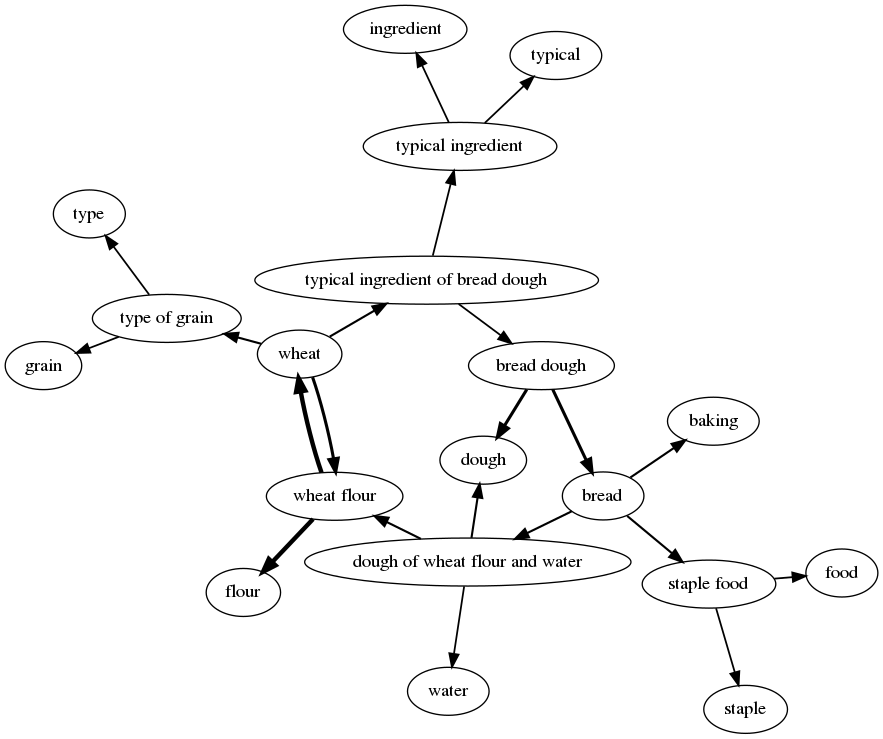
\includegraphics[width=\linewidth]{reports/technical_report/latex/figures/bread_graph-sections_only-implicit_references.png}
%     \caption{An example of a dependency-based graph created using the XML document from Figure \ref{fig:sample_xml_document}. Nodes represent the concepts that are referenced in the document. Edges in the graph represent the relationship `A references B'. Blue edges represent forward references and red edges represent backward references.}
%     \label{fig:graph_example}
% \end{figure}

\subsection{Identifying A Priori and Emerging Concepts} \label{sec:classifying_concepts}
To identify a priori and emerging concepts we can look at how the concepts are mentioned.
In particular, we could look for sentences that contain definitions.
One type of sentence that could be considered to contain a definition could be one that follows the pattern `X is a Y'.
If a concept appears as the subject of these kinds of sentences then perhaps that could indicate that the concept is an emerging concept.
For example, if the first mention of `SGX' is ``Intel Software Guard Extensions (SGX) is a set of security-related instruction codes that are built into some modern Intel central processing units (CPUs)'' then perhaps it is likely that SGX is being defined here and thus is an emerging concept.
We can look for other patterns in the structure of sentences that suggest that a concept is being defined, such `X is defined as a Y'.
The exact patterns that are used are described later in Section \ref{sec:rule-based_classifier}.
A priori concepts are then defined as any concept that does not fulfil the definition of an emerging concept.

%  It should be noted that this kind of approach would require knowledge of what kind of relations exist between concepts, a feature which has not been implemented yet in the current code. The current implementation works on the (incorrect) assumptions that: a concept that is only referenced from within a single section is an a priori concept; and concepts that are referenced from within multiple sections are emerging concepts. Implementing the method described in the previous paragraph is something to be looked at in future work.

% Placed here so the footer text appears on the same page
\begin{figure}
    \centering
    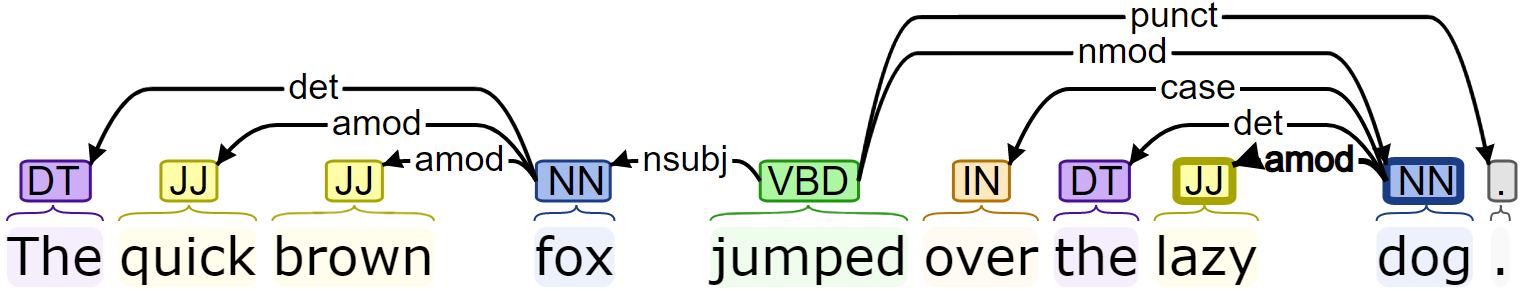
\includegraphics[width=\linewidth]{reports/technical_report/latex/figures/dependency_parse.png}
    \caption{An example of a dependency parse.\protect\footnotemark The arc labelled ``nsubj'' points to the subject of the sentence.
    For a description of what the relations on the arcs mean, refer to \citep{martin2018speech}.}
    \label{fig:dependency_parse_example}
\end{figure}

\footnotetext{
    Figure generated from \url{https://corenlp.run/}.
}

\subsection{Identifying Forward and Backward References} \label{sec:identifying_references}
In the graph, forward and backward references can be found through traversing the graph structure and identifying when the traversal algorithm crosses between document sections. A prerequisite is that we must record the sections that appear in the text, the order in which they are introduced during the parsing of the text document, and associate each node in the graph with a section. Each node is associated with the section that the node's corresponding concept appears in most frequently. In the case of a tie, the section that appears first is chosen. We can then identify a forward reference when the traversal algorithm visits a node that is associated with a section that comes after the section of the previously visited node. Similarly, backward references can be identified when the traversal algorithm visits a node that is associated with a section that comes before the section of the previously visited node. References are restricted to only point to nodes that have been labelled as emerging concepts since the definition of forward and backward references precludes references to a priori concepts. Pseudocode for this process is given in Algorithm \ref{alg:mark edges}.

\SetKwProg{Fn}{Function}{}{end}
\SetKwFunction{FMarkEdges}{markEdges}
\DontPrintSemicolon

\begin{algorithm*}
    \caption{Marking Forward and Backward References}
    \label{alg:mark edges}
    \KwData{
        $sections$: List of sections in a given document $D$ \\
        $nodes$: Set of nodes in the graph $G$ \\
    $nodes_\text{emerging}$: Set of nodes in $G$ labelled as emerging concepts \\
        $adj$: Adjacency list for a directed graph $G$.\\
    }
    \;
    $visited = \emptyset$\;
    \;
    \For{$node \in$ nodes}{
        markEdges($node$, NULL, visited)\;
    }
    \;
    \Fn{\FMarkEdges{curr, prev, visited}}{
        \tcc{
            Arguments\\
            curr: Current node\\
            prev: The previously visited node\\
            visited: Set of visited nodes
        }
        \;
    \uIf{$prev \neq NULL$ AND $curr.section \neq prev.section$ AND curr $\in nodes_\text{emerging}$}{
            \tcc{Find the ordering of the sections associated with the nodes $curr$ and $prev$.}
            $curr\_i \gets sections.indexOf(curr.section)$\;
            $prev\_i \gets sections.indexOf(prev.section)$\;
            \;
            \uIf{$curr\_i < prev\_i$}{
                Mark edge $\{prev, curr\}$ as a backward reference\;
            }
            \uElseIf{$curr\_i > prev\_i$}{
                Mark edge $\{prev, curr\}$ as a forward reference\;
            }
    }
        \;
        \uIf{$curr \notin visited$}{
            $visited \gets visited \cup \{curr\}$\;
            \;
            \For{neighbour $\in$ adj[curr]}{
                markEdges(\textit{neighbour, curr, visited})\;
            }
        }
    }
\end{algorithm*}

% \subsection{Cycles}
% We can also consider the number and length of cycles in the graph. Cycles in a graph would suggest the existence of self-referential loops in the text document - in other words sets of concepts that are defined in terms of themselves. Long cycles are perhaps not of too much concern since a long cycle may not necessarily encode a strong dependency between all of the concepts in the cycle. Short cycles, on the other hand may be indicative of strong interdependence and may prove difficult to learn the corresponding concepts since learning one of the concepts in isolation may not suffice.

% \subsection{Isolated and Disjoint Subgraphs}
% The idea of identifying bottlenecks in the graph structure can be extended to finding subgraphs that form isolated/disjointed clusters. Isolated clusters would be a set of interconnected vertices that have a small number of edges connecting them to the rest of the graph. These clusters would likely represent areas of a knowledge domain that could be learned in relative isolation from the reset of the domain, as long as the bottleneck concepts are learned. Similarly, disjointed subgraphs would also denote a similar thing. The existence of these isolated clusters or disjointed subgraphs would imply lower conceptual density than the alternative - a highly interconnteced graph.

\subsection{Deriving a Numerical Score} \label{sec:quantifying_conceptual_density}
At the centre of conceptual density is the notion of the degree to which concepts are integrated. In a graph structure, this could be measured by looking at the connectivity of nodes. One useful measure may be the average outdegree:
\begin{equation} \label{eq:simple score}
    S_D = \frac{1}{|V|} \sum_{v \in V} \text{deg}^+(v)
\end{equation}
where $S_D$ is the score of the document $D$, $V$ is the set of vertices in a graph, and $\text{deg}^+(v)$ is the outdegree, or the number of outgoing edges from the vertex $v$. The interpretation of a high average degree is that the average concept is relatively difficult to learn since the concept is related to many other concepts which you must understand to understand the given concept.

We can further refine the scoring method by taking into account the strength of the edges, or in other words the weights of the edges:
\begin{equation} \label{eq:weighed score}
    S_D = \frac{1}{|V|} \sum_{v \in V} \sum_{e \in E[v]} e_w
\end{equation}
where $E[v]$ is the set of edges originating from the vertex $v$, and $e_w$ is the weight for a given edge $e$.
% The previous formulation in Equation \ref{eq:simple score} can be thought of as a special case of this formulation where the weight for every edge is 1.
The weight for a given edge can be adjusted based on the type of reference the edge represents. For example, we could set the weight of an edge to: 1.0 for edges that point to a priori concepts since they typically represent a concept that the reader is expected to know beforehand and are easier to process; 1.5 for backward references to emerging concepts since the reader is required to recall a concept that has been introduced within the text and using a poorly integrated schema will require more mental exertion than when considering an a priori concept; and 2.0 for forward references since the reader is required to \textit{park} a new concept without anything concrete to pin it too, increasing cognitive load. The exact numbers are not important, but rather the relative scale of these numbers. References to a priori concepts should impose less cognitive load than backward references, and backward references should impose less cognitive load than forward references.

It should be noted that the scores generated by this model do not have much meaning on their own.
This is because it is difficult to come up with an interpretation of what a score of 3.1, for example, means in terms of conceptual density.
As such, the main purpose of these scores is for comparison and the scores should be interpreted as an ordinal scale.

\begin{figure}
    \centering
    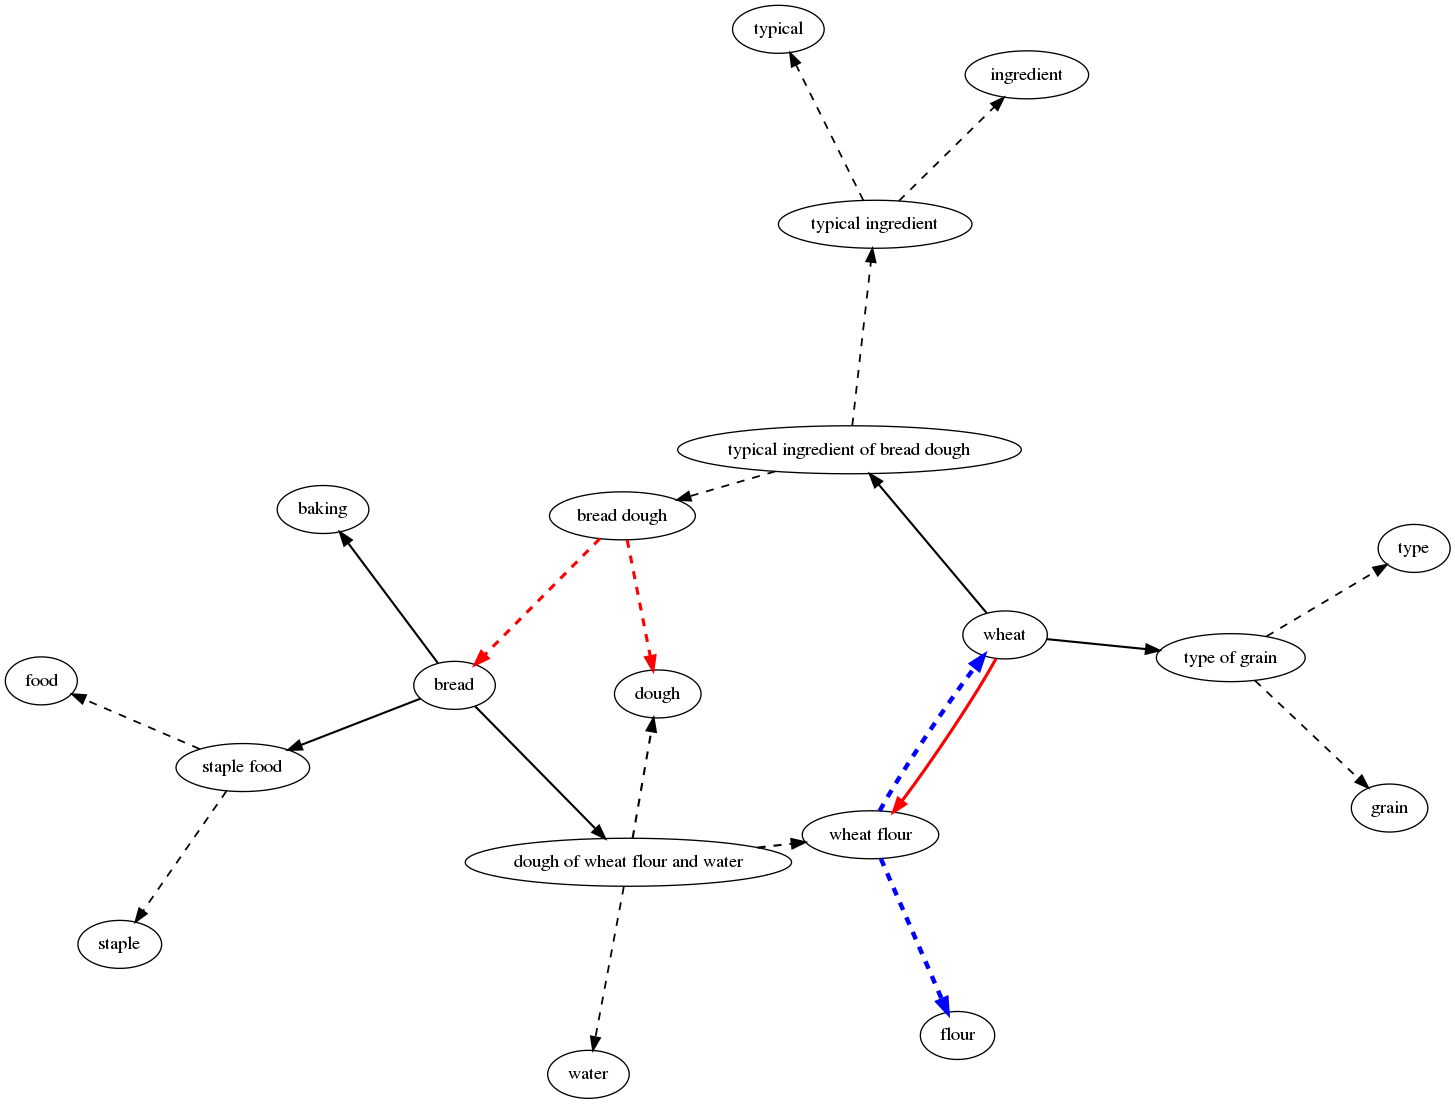
\includegraphics[width=\linewidth]{reports/technical_report/latex/figures/bread_graph-sections_only.png}
    \caption{An example showing the graph generated from the XML document in Figure \ref{fig:sample_xml_document} where forward and backward references have been coloured. Nodes represent the concepts that are referenced in the document. Edges in the graph represent a relationship between concepts. Blue edges represent forward references and red edges represent backward references.}
    \label{fig:graph_example-coloured_edges}
\end{figure}

\subsection{Summary}
By using part of speech tagging and a regex-based chunker we can extract concepts from text. We can then derive relationships between concepts by looking at dependency parses of sentence structures and by looking at the constituent parts of complex concepts represented by noun phrases. For the former method, we take the subject of a sentence and create edges between it and each of the other concepts that appear in the same sentence. Concepts are represented as a node in the graph and relationships between concepts are represented as edges in the graph.
The different types of concepts and references can be identified by analysing the edges in the graph. Finally, we can derive a score from the generated graph by measuring the average weighted outdegree. Figure \ref{fig:graph_example-coloured_edges} shows the graph generated using the current implementation and the sample text document in Figure \ref{fig:sample document}.

\section{Implementation of the Conceptual Density Model} \label{sec:implementation_of_the_conceptual_density_model}
In this section, I will describe the implementation of the model discussed across Sections \ref{sec:conceptual_density_in_text} and \ref{sec:building_a_graph_of_concepts} that is used in the experiments. The current implementation takes in a XML formatted document, parses the document and extracts concepts and relations between concepts, builds up a graph representation of these extracted entities and generates a score. The way the score is generated is the same as it was described in Section \ref{sec:quantifying_conceptual_density}, so I will only describe the other aspects below.
Also, since the motivation and rationale for the different aspects of the model are explained in the previous sections, I will focus on describing the steps involved in processing a document in more detail. The source code for the model is made publicly available \cite{anthony_dickson_2019_3474469}.

\subsection{Input Format}
One limitation of the current implementation is that documents must be marked up in XML. The reason why this semi-structured text format was chosen is that identifying sections and where start and end in plain text is not always reliable (this is discussed briefly in Section \ref{sec:future_work}, Future Work) and it is of interest to see how the model performs assuming sections can be identified correctly. The format as is follows: the root element is a \texttt{document} element; each section is enclosed within a \texttt{section} element and nested sections are lifted up to be a child of the root node, rather than the parent section in the text (this is not by design, but rather a limitation of the current implementation); the title of each section is enclosed within a \texttt{title} element inside the corresponding \texttt{section} element; and the text of each section is enclosed within a \texttt{text} element inside the corresponding \texttt{section} element.
An example is shown in Figure \ref{fig:sample_xml_document}.


\subsection{Parsing Algorithm} \label{sec:parsing_algorithm}
The parsing algorithm is the part of the model that analyses the text. It extracts the concepts (nodes) and relations between concepts (edges) and inserts them into the graph. There are three main stages to the parsing algorithm: parsing the DOM (document object model) from the input XML; extracting concepts and relations between concepts from the text of each section; performing post-processing on the resulting graph to normalise/fix it. The algorithm is as follows:
\begin{enumerate}
    \item Parse the input XML file and generate the document object model (DOM).
    \item For each section element in the DOM:
    \begin{enumerate}
        \item Extract the title from the title element and convert it to lowercase.
        \item Extract the text from the text element and convert it to lowercase.
        \item Split the text into sentences.
        \item For each sentence:
        \begin{enumerate}
            \item Tokenise the sentence into white-space separated words.
            \item Tag each token with its part of speech (POS).
            \item Normalise tokens by replacing them with their lemmas (the non-inflected/dictionary form of a word).
            \item Analyse the dependency tree of the sentence to find the subject of the sentence.
            \item Optionally, analyse the dependency tree of the sentence and look for emerging concepts using a rule-based classifier (discussed below).
            \item Chunk the POS tagged tokens using the grammars defined in Section \ref{sec:idenifying_concepts} to create a constituency tree.
            \item Extract the concepts identified by the grammars and insert the concept representing the subject and each extracted concept into the graph. Also create an edge between the subject and the extracted concepts.
            \item Add constituent concepts of complex noun phrases to the graph in a similar way as above.
        \end{enumerate}
    \end{enumerate}
    \item Perform post-processing steps on the resulting graph:
    \begin{enumerate}
        \item Assign a section to each concept - this represents where the concept was defined in the text.
        \item Classify concepts as either a priori or emerging using a graph-based approach (described below). Only concepts that were not classified in the earlier steps are classified in this step.
        \item Filter emerging concepts based on their word frequency (described below).
        \item Mark forward and backward references using the method described in Section. \ref{sec:building_a_graph_of_concepts}. This method only works for edges between distinct nodes in the graph. Additional edges are added for concepts that are referenced verbatim (i.e. referenced in the same form) in preceding or following sections.
    \end{enumerate}
\end{enumerate}

\subsubsection{Assigning Sections to Nodes}
In regards to step 3a, where a concept is defined in a given text is decided upon with the simple assumption that a concept is mentioned the most in the section that it is defined in (although this may not always be the case). This step is mainly for ensuring that forward and backward references are assigned more accurately in later steps, and as such is only relevant for emerging concepts.
There are some cases where this method does not produce the correct results.
For example, in the sample text on bread in Figure \ref{fig:sample_txt_document}, wheat flour is mentioned in the first section but not defined until the following section and the concept is mentioned once in each section. The first mention of the concept should create a forward reference. However, based on how nodes in the graph are assigned to a section (refer to Section \ref{sec:identifying_references}), the concept `wheat flour' would be assigned to the first section (due to the tie break condition) and thus the second time `wheat flour' is mentioned it creates a backward reference to the mention in the first section. This particular case and similar cases can be corrected for by first observing that the concept appears in the title of a section, and assigning the concept to the section whose title contains the concept.

\subsubsection{Filtering Emerging Concepts}
For all of the methods described below, emerging concepts are filtered by their word frequency using the Zipf scale \citep{brysbaertzipf, van2014subtlex} to help prevent common words being misclassified as emerging concepts.
If a classifier has decided to label a concept as an emerging concept, only concepts that are below the threshold value are accepted as emerging concepts, otherwise the concept is labelled as an a priori concept.
This threshold value was set to 3.0.
This value was found empirically by experimenting with different values and choosing the threshold value that gave the best results in experiments (see Sections \ref{sec:entity_recognition} and  \ref{sec:entity_recognition_results} for the methodology and results of the experiment in question).

\subsection{Comparing Methods for Classifying Concepts}
In the experiments four different approaches to classifying concepts are evaluated: a graph-based classifier, a rule-based classifier, a classifier that combines the graph-based and rule-based classifier, and a random classifier. These are described below.

\subsubsection{Graph-Based Classifier}
This approach classifies concepts using the graph topology. This approach works on the sometimes incorrect assumptions that: a concept that is only referenced from within a single section is an a priori concept; and concepts that are referenced from within multiple sections are emerging concepts. This is implemented by looking at the incoming edges for a given node and for the tail of each of these edges counting the number of distinct sections that these tail nodes belong to. Then we make a simple decision, if the number of sections is one then the concept/node is labelled as an a priori concept, otherwise if the number of sections is greater than one the concept is labelled as an emerging concept.

As alluded to above, there are cases where these assumptions do not hold.
Using the Wikipedia article on closures \citep{wiki:closure} as an example, the concept ``closure operator'' is referenced from multiple sections and is indeed an emerging concept.
However, the concept ``set'' is referenced from multiple sections however it is not an emerging concept as the method might suggest.

It may be strange that this is being included even though it is based on incorrect assumptions. However, interesting results are produced when compared against an approach that is more faithful to the method described in Section \ref{sec:classifying_concepts}.

\subsubsection{Rule-Based Classifier} \label{sec:rule-based_classifier}
This approach is intended as the first steps to address the issues of the graph-based approach and improve the accuracy of the concept classification.
In this approach the algorithm analyses dependency trees and matches simple patterns to pick out concepts that look like they are being defined (i.e. the concept is likely an emerging concept).
The basic patterns that are matched are:
\begin{itemize}
    \item Subjects of sentences where the main verb is `be' and the object is a NP.
    For example, in the sentence ``Apples are a type of fruit.'', ``Apples'' would be labelled as an emerging concept.
    \item Sentences where the main verb is `define':

    \begin{itemize}
        \item Direct objects of sentences where the verb `define' is used in the active voice.
        For example, in the sentence `These three properties define an abstract closure operator.'', ``abstract closure operator'' is labelled as an emerging concept.
        \item Subjects of passive sentences where the main verb is 'define'.
        For example, in the sentence ``The congruence closure of R is defined as the smallest congruence relation containing R.'', ``congruence closure of R'' is labelled as an emerging concept.
    \end{itemize}

    \item Objects of passive sentences where the main verb is `call'.
    For example, in the sentence `This smallest closed set is called the closure of S ...'', ``closure of S'' would be labelled as an emerging concept.

\end{itemize}

\subsubsection{Composite Classifier}This approach is a synthesis of the graph-based and rule-based classifiers.
In this approach the rule-based classifier takes precedence, and any concepts not classified by it are then processed by the graph-based classifier.

\subsubsection{Random Classifier} This approach labels concepts as a priori or emerging randomly with equal probability. Since there are no benchmarks to compare the other approaches for classifying concepts with, the next best thing is to compare it against is a classifier that assigns labels randomly. This approach is intended to serve as a baseline to compare the other methods against.

\section{Evaluation} \label{sec:evaluation}
In this section, I will discuss how the quality of the model for quantifying conceptual density is evaluated.
For evaluating the quality of the parsing algorithm, the extracted concepts and relations between concepts for a given document are compared against a set of annotations for that document.
Then, we look at how the scores generated by model change as the order of the sections in a document are permuted.
In the last experiment, a set of three documents are ranked in order of least to most conceptually dense based on human judgements and compared against the ranking produced by the model.
First, I will describe the annotation process, then following that I will describe the setup for the three experiments and finally I will discuss the results for each of these experiments.

\subsection{Annotated Document} \label{sec:annotated_document}
The Wikipedia article on closures \citep{wiki:closure} was annotated with concepts (a priori and emerging) and references (forward and backward).
A web-based tool was created to facilitate the creation of annotated documents and to automate the process of generating an XML version of the annotations for the evaluation scripts to use as input. The source code for this annotation tool is made publicly available \citep{anthony_dickson_2019_3458618}.

Two approaches were taken when creating the annotations which targeted \textit{low-level concepts} and \textit{high-level concepts} separately.
The idea of a low-level concept refers to an \textit{atomic concept}, a concept that is named using a single token.
Conversely, a high-level concept refers to a \textit{compound concept}, a concept that is named using one or more tokens.
For example, `
The idea of a high-level concept is similar to that of the complex noun phrases mentioned in Section \ref{sec:idenifying_concepts}.
% To clarify, the uses of `low-level' and `high-level' refer to the level of syntactic structure, rather than the semantic type hierarchy.
The reason why both approaches are used is that for a given phrase/sentence, there is not necessarily only one set of correct annotations.
For example, in the phrase ``A set is closed under an operation ...'' it is clear that `set' is a single, atomic concept. However, the same may not be able to be said about the verb phrase `closed under an operation'. One could argue there are two concepts, `closed' and `operation'. However, one may also argue that `closed under an operation' forms a single, composite concept that has a meaning distinct from the constituent concepts in isolation. How do we reconcile these different approaches? We could just choose one approach over the over, but we would risk losing potentially important information.
To this end, the two sets of annotations that target low-level concepts and high-level concepts were created.
These two sets of annotations are concatenated and used as the ground truth set of annotations for the purposes of evaluation.
See Table \ref{tab:annotations_distribution} for the distribution of the annotations and Figure \ref{fig:annotatations_sample} for an example of some high-level concept annotations.

\begin{table}
    \centering
    \begin{tabular}{|l|r|}
        \hline
        A Priori Concepts & 257  \\
        Emerging Concepts & 94 \\
        Concepts Total & 351 \\
        \hline
        Forward References & 3 \\
        Backward References & 10 \\
        References Total & 13 \\
        \hline
        Annotations Total & 364 \\
        \hline
    \end{tabular}
    \caption{Counts for different types of annotations in the closures document.}
    \label{tab:annotations_distribution}
\end{table}

\begin{figure}
    \centering
    \includegraphics[width=\linewidth]{reports/technical_report/latex/figures/annotations-sample.png}
    \caption{A sample of the annotations for the Wikipedia article on closures. The sections highlighted gray indicate a priori concepts and the section highlighted green indicate emerging concepts.}
    \label{fig:annotatations_sample}
\end{figure}

These annotations were checked by my two supervisors and any discrepancies were discussed and resolved accordingly in a rather ad hoc manner.
However, in future work it would be best if documents are annotated independently by multiple judges so that inter-rater reliability can measured through something like Cohen's Kappa coefficient \citep{cohen1960coefficient, mchugh2012interrater}, for example. This would allow for the quality of the annotations to be assessed in a principled manner.

\subsection{Entity Recognition} \label{sec:entity_recognition}
The first experiment looks at evaluating the quality of the parsing algorithm and its ability to correctly extract concepts and identify forward and backward references.
We can characterise the parsing algorithm as an algorithm that tries to predict the ground truth set of annotations for a given document. The ground truth set of annotations for a given document are the distinct concepts and references from the corresponding annotated version of the document.
We can evaluate the quality of the parsing algorithm by calculating metrics on the predicted set of annotations generated by it. The metrics used are precision, recall and the $\text{F}_1$ score (the harmonic mean of recall and precision). These metrics are calculated for each type of concept (a priori and emerging) and each type of reference (forward and backward).
Additionally, these metrics are calculated for the four different approaches to classifying concepts described in Section \ref{sec:parsing_algorithm}.
The results for this experiment are discussed in Section \ref{sec:entity_recognition_results}.
Other, alternative parsing algorithms for entity recognition are also evaluated.
However, these approaches are not the main focus of this report and as such these approaches and their results are briefly discussed in Appendix \ref{sec:alternative_parsers}. Below I will briefly define and discuss the metrics used in this experiment.

\subsubsection{Definition of Metrics}
\paragraph{Precision} In binary classification, precision is defined as the proportion of samples labelled as \textit{positive} by a classifier that are actually positive.
Positive may refer to the presence of something as opposed to the absence of something (e.g. in image classification, the presence of a cat in an image from a set of images containing cats and dogs where the task is to identify cats), or more generally, it may simply refer to one of the two classes in the binary classification problem.
Precision can be interpreted as how reliable a classifier is when it labels a sample as positive.
Following on the from the previous example, precision could answer the question: out of the $n$ samples some classifier labels as cats, how many samples are actually of cats? Precision can defined mathematically as the number of elements in the intersection between the set of ground truth labels and the set of predicted labels for positive samples, divided by the number of elements in the set of predicted labels for positive samples:
\begin{equation*}
    p = \frac{|t \cap y|}{|y|}
\end{equation*}
where $t$ is the ground truth set of positive labels and $y$ is the predicted set of positive labels.

\paragraph{Recall} Recall is a measure of the proportion of positive samples that a classifier was able to identify out of all positive samples. Recall can be interpreted as how thorough a classifier is in identifying all instances of a given class. Using the example of classifying images of cats and dogs, recall could answer the question: out of the $n$ cats in the data set, how many cats was the classifier able to identify/label as cats? Recall can defined mathematically as the number of elements in the intersection between the set of ground truth labels and set of predicted labels for positive samples, divided by the number of elements in the set of ground truth labels for positive samples:
\begin{equation*}
    r = \frac{|t \cap y|}{|t|}
\end{equation*}
where $t$ is the ground truth set of positive labels and $y$ is the predicted set of positive labels.

\paragraph{$\text{F}_1$ Score} $\text{F}_1$ score is the harmonic mean of precision and recall. It summarises precision and recall in a single metric and is calculated as such:
\begin{equation*}
    \text{F}_1 = 2 \frac{p r}{p + r}
\end{equation*}
where $p$ is precision and $r$ is recall. One characteristic of the harmonic mean is that it punishes extreme values more heavily in comparison to the arithmetic mean. For example, consider a precision and recall of 0.1 and 0.9. The arithmetic mean for these would be 0.5, however the harmonic mean would be 0.18.

\subsection{Permuting the Order of Sections}
The second experiment looks at evaluating the scores generated by the conceptual density model and how sensible these scores are when the order of sections in a document are permuted.
% The assumption is that expository documents are written in an optimal manner that facilitates easy understanding of the content and that concepts are explained/introduced in an order that minimises the number of forward references (since forward references cost the most in terms of conceptual density). This is a way to evaluate the quality of the model without human judgements.
The assumption is that the author of an expository text chooses to introduce concepts/topics (sections) in an order that is easy to read and understand, and by permuting the order of the sections in the text we expect the text to become more difficult to read and understand.
% For example, consider an introductory programming textbook that, among other concepts, introduces the concepts of functions and recursion, in that order. Now imagine the effect of introducing recursion before functions, no doubt it would be difficult to understand.
In terms of the conceptual density model, permuting the order of sections will change the number of forward and backward references (however, it does not change the total number of references) based on the new section order (recall that whether a reference is considered a forward or backward reference is dependent on the relative order of sections).
Due to the way references are weighted in the graph, the score generated by the model will also change as the sections are permuted.
Hence, we can expect the model to reflect the change in readability of a given text through the scores that it generates as the sections are permuted, and by measuring these scores for different permutations we can evaluate the quality of the model without the need for human judgements.
However, it should be noted that this method of evaluation does not necessarily directly measure the quality of the model in regards to conceptual density, rather it is a proxy that measures something like a readability score. The results for this experiment are discussed in Section \ref{sec:permuting_the_order_of_sections_results}.

% We would expect the score given by the model to change when the order of the sections are changed. This is because changing the order of sections will also change forward references to backward references and vice versa depending on the new order of the sections. Due to how references are weighted in the graph, changing forward references to backward references to decrease the score of conceptual density and increase it when changing backward references to forward references.

\subsection{Ranking Documents} \label{sec:ranking_documents}
Although there is no existing gold standard when it comes to evaluating models of conceptual density, we can evaluate the model against human judgements and intuition. In this experiment, the task is to rank a set of three Wikipedia articles \citep{wiki:habsburg, wiki:cdo, wiki:dna} from least to most conceptually dense. The documents were selected such that they all had roughly the same length and that there was a document for each of low, medium and high conceptual density.

Human judgements (rankings) were gathered by having each judge ($n=3$) independently read the documents and rank them based on pre-theoretical assessments of conceptual density. Each judge was given a brief description of conceptual density to base their assessments on before starting. This description is as follows: ``A tightly integrated concept is a concept that is difficult to describe or explain independently of other concepts''.
All judges reached the unanimous agreement that the ranking of the three documents based on this definition from least conceptually dense to most conceptually dense is as follows: House of Habsburg \citep{wiki:habsburg}, CDO \citep{wiki:cdo} and then DNA \citep{wiki:dna}. One thing to note is that the three judges were the two supervisors for this project and myself.
This is perhaps not ideal since all judges were aware of the hypothesis being tested beforehand.
Ideally for future work, documents would be ranked by judges with little to no exposure to the hypothesis being tested.

A ranking of the documents is derived from the model by generating a score for each document and then sorting by the scores.
The results for this experiment are discussed in Section \ref{sec:ranking_documents_results}

\subsection{Results}
\subsubsection{Entity Recognition} \label{sec:entity_recognition_results}
The conceptual density model was evaluated on the set of annotations for the Wikipedia article on closures as described in Section \ref{sec:annotated_document} and the results are listed in Figure \ref{fig:parser_results}.
Denoted by `Random' in the results table is the random classifier.
Metrics that are calculated for the random classifier are reported with the mean and the margin of error representing the 95\% confidence interval calculated from 40 independent trials.
Denoted by `Graph-Based' is the graph-based classifier, denoted by `Rule-Based' is the rule-based classifier and denoted by `Composite' is the composite classifier.

\begin{figure}
    \centering
    \begin{subfigure}[b]{\textwidth}
        \caption{Precision}
        \label{fig:precision}
        \centering
        \begin{tabular}{|l|r|r|r|r|}
            \hline
            {} & Random & Graph-Based & Rule-Based & Composite \\
            \hline
            A Priori Concepts & 0.361 ($\pm$ 0.008) &        \textbf{0.404} & 0.396 & 0.361 \\
            Emerging Concepts & 0.120 ($\pm$ 0.005) & 0.164 & 0.165 &      \textbf{0.170} \\
            \hline
            Forward References & 0.024 ($\pm$ 0.007) &        \textbf{0.043} &       \textbf{0.043} &     \textbf{ 0.043} \\
            Backward References & 0.067 ($\pm$ 0.008) & 0.066 & 0.075 &      \textbf{0.085} \\
            \hline
        \end{tabular}
    \end{subfigure} \\
    \begin{subfigure}[b]{\textwidth}
        \caption{Recall}
        \label{fig:recall}
        \centering
        \begin{tabular}{|l|r|r|r|r|}
            \hline
            {} & Random & Graph-Based & Rule-Based & Composite \\
            \hline
            A Priori Concepts &  \textbf{0.302 ($\pm$ 0.009)} & 0.237 & 0.222 & 0.206 \\
            Emerging Concepts & 0.277 ($\pm$ 0.014) & 0.489 & 0.511 &      \textbf{0.521} \\
            \hline
            Forward References & 0.278 ($\pm$ 0.083) &        \textbf{0.667} &       \textbf{0.667} &      \textbf{0.667} \\
            Backward References & 0.337 ($\pm$ 0.039) & 0.500 & 0.600 &      \textbf{0.700} \\
            \hline
        \end{tabular}
    \end{subfigure} \\
    \begin{subfigure}[b]{\textwidth}
        \caption{$\text{F}_1$ Score}
        \label{fig:f1_score}
        \centering
        \begin{tabular}{|l|r|r|r|r|}
            \hline
            {} & Random & Graph-Based & Rule-Based & Composite \\
            \hline
            A Priori Concepts &  \textbf{0.329 ($\pm$ 0.008)} & 0.299 & 0.284 & 0.262 \\
            Emerging Concepts & 0.168 ($\pm$ 0.007) & 0.246 & 0.249 &      \textbf{0.257} \\
            \hline
            Forward References & 0.066 ($\pm$ 0.008) &        \textbf{0.080} &       \textbf{0.080} &      \textbf{0.080} \\
            Backward References & 0.111 ($\pm$ 0.013) & 0.116 & 0.133 &      \textbf{0.152} \\
            \hline
        \end{tabular}
    \end{subfigure}
    \caption{Tables showing results from evaluating the parsing algorithm on annotations from the closures document. Results are rounded to three decimal places and the best method for classifying a priori and emerging concepts are emphasised in bold. The results for the `Random' classifier calculated from 40 independent trials are reported as the mean and in parentheses the margin of error (95\% confidence interval).}
    \label{fig:parser_results}
\end{figure}

Overall, the graph-based classifier, the rule-based classifier, and the composite classifier are more accurate than the random classifier in most cases by a small margin. The only cases where the random classifier outperforms these three classifiers is for the recall and $\text{F}_1$ scores calculated on a priori concepts.
Notably, for precision the margin between the three methods and random is small, ranging between -0.01\% and 4.3\%. The margin between the three methods and random is larger when it comes to recall, ranging between -9.6\% and 38.9\%. For $\text{F}_1$ score, the margin between the three methods and random is not as extreme, ranging between -6.7\% and 8.9\%.
There is no single approach that always performs the best out of the four methods evaluated, however it appears that the composite classifier performs the best most of time.

There are a few reasons why the implementation of the model does not perform too well at identifying concepts:
\begin{itemize}
    \item The parser does not handle actions (verbs and verb phrases) and thus fails to identify many concepts.
    \item The parser does not always chunk tokens in the same way as tokens are chunked in the annotations, e.g. `\textit{thus a} subgroup of a group' produced by the model instead of `subgroup of a group' in the annotations.
    \item For the rule-based classifier, the set of rules is rather simplistic and far from exhaustive.
    For example, it fails to recognise that the concept `closed' is being defined in the sentence ``A set is closed under an operation if ...''.

    \item Particular to documents that contain equations, the way that how equations are parsed produces many spurious/meaningless tokens which adds noise and lowers precision. In the case of the composite classifier, about 35 of the extracted concepts are such tokens.
\end{itemize}

Despite the reasonable recall for references (although note the small samples size of 13), all methods result in low precision, at best 4.3\% and 8.5\% for forward and backward references, respectively. This is likely due to the fact that the current implementation identifies many more forward/backward references (116 and 141, respectively) in comparison to the actual number of references (3 and 10, respectively).

One explanation for why the parser produces too many references may be that due to the low precision of the concept classifiers, highly frequent concepts that are mentioned across many sections are erroneously marked as emerging concepts, which in turn would produce many references. One such example is the concept `set' in the article on closures. The model erroneously marks the concept as an emerging concept and the concept is referenced from every section by a total of 43 different concepts. Of these 43 references to the concept `set', 14 create a forward reference, 19 create a backward reference, and 10 occur in the same section and thus create neither a forward or backward reference.
So due to the parsing algorithm marking `set' as an emerging concept, 33 references are incorrectly identified.
Removing these references from the predicted set of references would increase precision by at most 0.6\% and 1.3\% for forward and backward references, respectively.
While this is the most extreme example, we can imagine how the quality of the set of forward and backward references would be adversely affected by having many concepts misclassified as emerging concepts, and how the metrics would improve if the classification of concepts was made more accurate.
% One thing to keep in mind about the results for references is the small sample size of 13 of which three are forward references and 10 are backward references. \todo{Why does this matter?}

\subsubsection{Permuting the Order of Sections} \label{sec:permuting_the_order_of_sections_results}
For this experiment, the Wikipedia article on closures \citep{wiki:closure} is used.
For reference, the sections in their original order are: `closure (mathematics)', `basic properties', `closed sets', `examples', `closure operator' and `binary relation closures'.
Ideally, we would expect the model to generate the lowest score for this ordering.
However, based on the current model the only thing that changes as sections are permuted is the assignment of forward and backward references.
Hence, we expect the model to generate the lowest score for the ordering that minimises the ratio of forward references to backward references (forward references have larger weights than backward references).
Based on these assumptions and the annotations for the closures article, the expected order of sections that give the lowest conceptual density could be:
`closure (mathematics)', `closure operator', `closed sets', `basic properties', `examples', `binary relation closures'.
This ordering makes intuitive sense for the most part since sections that build upon concepts introduced in the article are placed towards the end.

The section ordering with the lowest and highest conceptual density given by the model were:
\begin{itemize}
    \item lowest score of 2.31: `closed sets', `examples', `closure operator', `basic properties', `closure (mathematics)', `binary relation closures'
    \item highest score of 2.43: `binary relation closures', `closure (mathematics)', `basic properties', `closure operator', `examples', `closed sets'.

\end{itemize}

These results, while not exactly what was expected, are still somewhat intuitive. For the ordering with the lowest conceptual density, the section that explains the main topic/core concept is first and the section that seems to me to be the most conceptually dense is last. However, it is odd that the introductory section is placed second to last in the ordering that gives the lowest conceptual density.

We can reason about why the ordering given by the model does not match the expected ordering.
The only thing that changes as we permute the sections is which references are marked as forward references and which references are marked as backward references.
Thus, the reason why the output from the model does not match the expected output is that the model has not identified the set of forward and backward references that matches the set of references present in the annotations upon which the expected orderings are based on.
Simply by comparing the number of references identified by the model (264) to the number of references present in the annotations (13), it is clear that this is the case.
If the portion of the parsing algorithm that identifies references is improved, then the model would give results that are closer to what we would expect.

One may notice that there is only a difference of 0.12 between the ordering that gives the lowest conceptual density and the ordering that gives the highest conceptual density.
The small difference is due to these main factors:
\begin{itemize}
    \item Reordering the sections only changes the number of forward and backward references, and the weights for these only have a difference of 0.5.
    \item The scores are the average weighted outdegree of the generated graph, and there are only a few forward and backward references (3 forward references and 10 backward references across annotations for both low-level and high-level concepts) and many nodes in the graph (436) so the difference is small.
    \item The parser misses some forward and backward references which makes the difference even smaller.
\end{itemize}

\subsubsection{Ranking Documents} \label{sec:ranking_documents_results}
The ranking produced by the model for the three Wikipedia articles \citep{wiki:habsburg, wiki:cdo, wiki:dna} is as follows, with scores in the parentheses: DNA (2.62), CDO (2.66), House of Habsburg (2.94).
As previously stated, the expected ranking of the three articles is:
House of Habsburg, CDO and then DNA.
We can see that the model has produced results that are the opposite of the expected ordering.
The main contributor to the model producing the opposite ranking is, by the very definition of the scoring algorithm, the average outdegree of the graph.
The average outdegree, rounded to two decimal places, for the graphs generated for each document are: DNA (1.97), CDO (2.02) and House of Habsburg (2.14).
Based on the rankings and definition of conceptual density, neither these numbers or the reverse order of the expected rankings are expected.
Why is it the case that the document judged to have the lowest conceptual density has the highest score and average outdegree?

There are a couple of possible reasons for why the model produces the incorrect rankings that come to mind.
It could be that the human judgements capture something that is not quite in line with the notion of conceptual density that the model is based on. For example, it could be that judges are ranking documents based on a notion that is most similar to a measure of readability.
Another explanation could be that the writing styles for the documents differ in a way that biases the scores. For example, perhaps it is the case that in the article on the House of Habsburg is written in a way that means on average more concepts are mentioned within a sentence.
This hypothesis is supported by looking at the average sentence length (in number of tokens) for each document.
Rounded to one decimal place, the article on the House of Habsburg has on average 22.3 tokens per sentence, the article on CDOs 20.6 and the article on DNA 18.9.
The fact that the final score reflects the structure of sentences is not surprising; the way that concepts are related is dependent on sentence structure (see Section \ref{sec:edges_and_relating_concepts}).

This suggests two things: something in the implementation needs fixing; and the length of sentences needs to be controlled for in some way.
There is some evidence for the former point. For example, in the graph generated for the sample text given in Figure \ref{fig:sample_txt_document}, an edge is created between `wheat' and `typical ingredient of bread dough' (see Figure \ref{fig:graph_example-coloured_edges}). However, looking at the text and the structure of that sentence, it is clear that the concept `typical ingredient of bread dough' is being mentioned in reference to the concept `wheat flour', not `wheat'.
Adjusting the way concepts are related to be more `concept-centric' (as opposed to the current `subject-centric' approach) would weaken the correlation between sentence length and the scores and perhaps shift the scores in a way that makes the expected ranking more likely to be produced by the model.

Despite producing the opposite of the expected ranking, looking at the data produced by the model there is also indication that different scoring schemes could produce the expected ranking. One case where the predicted ranking would match the expected ordering:

\begin{itemize}
    \item ordering documents by the ratio of nodes to edges, which is like the inverse of the average outdegree (numbers in parentheses correspond to the number of nodes, edges and the ratio of nodes to edges):
    \begin{itemize}
        \item House of Habsburg (2034/4351/0.47)
        \item CDO (1778/3596/0.49)
        \item DNA (2451/4823/0.51)
    \end{itemize}
\end{itemize}

One alternative ranking that was also proposed was: CDO, House of Habsburg, DNA.
There is one case where the predicted ranking would match the this ordering:
\begin{itemize}
    \item ordering documents by number of emerging concepts when using just the rule-based concept classifier (numbers in parentheses correspond to the number of emerging concepts):
    \begin{itemize}
        \item CDO (1223)
        \item House of Habsburg (1506)
        \item DNA (1669)
    \end{itemize}
\end{itemize}

While promising, these observations may not hold as the parsing algorithm is made more accurate. However, it does raise the question of whether or not the assumptions that the current scoring algorithm is based upon are all correct.

\subsection{Summary}
In this section, I have described how annotations of documents can be created and methods for evaluating the conceptual density model. The current implementation of the conceptual density model was evaluated with the methods described in this section and the results were discussed. The main takeaway from the results is that much of the model is heavily dependent on how accurately concepts are identified, and as such future work should prioritise improving the parsing algorithm and the identification of concepts.

\section{Related Work} \label{sec:related_work}
\subsection{Information Extraction}
The process of identifying concepts and how they are related that I have described in this report is similar to the task of information extraction. However, there are some key differences between what I have done and what is usually done in information extraction. First and foremost, information extraction seems to typically be concerned with named-entity recognition - the identification of named-entities such as names of people, companies, locations, and dates. In this study, we are concerned with concepts in general (all types of entities), which can be thought of as a superset of named-entities. Furthermore, information extraction is also interested in the relationship between named-entities. However, in the work-to-date, we have not been not too concerned about the nature of a relationship between concepts as much as the fact that a relationship exists.

\subsection{Semantic Networks and Knowledge Graphs}
The type of graph structure that is being built up in the conceptual density model is very similar to semantic networks/knowledge graphs. Some differences between the graphs produced by the conceptual density model and semantic networks are that: we are not annotating edges with the type of relationship (compare Figure \ref{fig:graph_example-coloured_edges} and Figure \ref{fig:semantic_network_example}, for example), and the criteria for deciding what constitutes a node or edge in the graph may differ from what is common in the literature. For example, somewhat complex noun phrases are added as nodes in the conceptual density model rather than just simple noun phrases or the head of noun phrases.

\begin{figure}
    \centering
    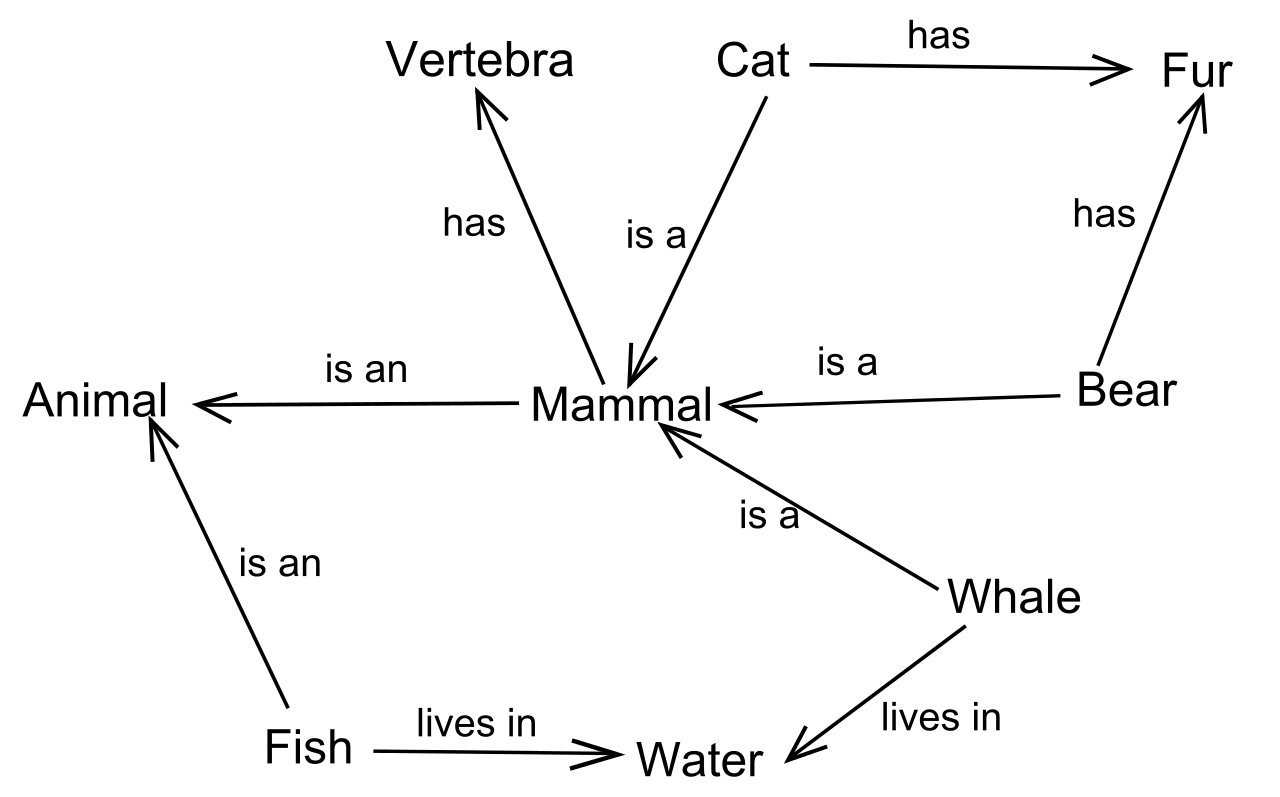
\includegraphics[width=\linewidth]{reports/technical_report/latex/figures/semantic_map_example.png}
    \caption{An example of a semantic network.\protect\footnotemark}
    \label{fig:semantic_network_example}
\end{figure}

\footnotetext{Figure from \url{https://commons.wikimedia.org/wiki/File:Semantic_Net.svg}.}

\section{Future Work and Open Problems} \label{sec:future_work}
\subsection{Suitability of Hypertext}
The model of conceptual density was evaluated on articles from Wikipedia. One possible issue is that the methods explored in this report depend on the linearity of a text. Textbooks are a linear medium of text since you are expected to read each page in order and all of the necessary information for understanding the current section is given ahead of time. In contrast, hypertext documents are not necessarily designed in the same way. Concepts are often hyperlinks which can be followed, and when they are followed it is fair to consider the flow of the original document broken and the original document no longer linear. One case where hypertext may be considered linear is where the reader is one who understands all of the prerequisite concepts and thus follows very few or even zero links when reading the hypertext.

\subsection{Type-Token Distinction}
Another issue is the distinction between types and tokens. We can think of types as classes and tokens as instances of a given type/class, e.g. Dunedin is a token/instance of the type/class `city'. An interesting question that arises is: should tokens be weighted differently from types - i.e. should tokens increase conceptual density as much types? Much of history talks about historical figures, is it difficult to understand what is going on even if we do not know exactly who the people being talked about are? In contrast, how likely is one to understand what a collateralised debt obligation or a mortgage backed security is if they do not know what an asset backed security is? It is more likely that one would be able to understand the interactions between historical figures (instances of people) than understand types of different tradeable financial assets even if they are already familiar with both people and asset backed securities.

Another issue is whether or not a token can be considered a concept at all. A concept is sometimes defined as an abstract idea or ``a mental representation of the essential or typical properties of something, considered without regard to the peculiar properties of any specific instance or example'' \citep{oxford_concept}. Assuming we accept this definition of a concept, then we could argue that tokens are in fact not concepts.

\subsection{Transitioning to Unstructured Text}
In the current implementation a graph can be built from semi-structured text (e.g. Figure \ref{fig:graph_example-coloured_edges}), but recreating the same graph from the corresponding plain text version of a document remains difficult. Moving to unstructured text is desirable since using semi-structured text requires someone to manually mark up the text which is a time-consuming process and requires them to adhere to a standard format, which is bound to be error-prone. At present, the sections and section headers must be explicitly marked up in XML. Identifying the section titles and where sections start and end automatically can be unreliable at times when using simple regex pattern matching due to different section heading formats and it is liable to false positives (see Table \ref{tab:section_finding_example} in the appendix, for example).

% \subsection{Classification of A Priori and Emerging Concepts}
% The naming and intent behind a priori and emerging concepts has changed quite a bit over time, and as such the current implementation (as described in Section \ref{sec:classifying_concepts}) for identifying the two types of concepts no longer produces the desired results. To more accurately distinguish a priori concepts from emerging concepts we could look at how concepts are mentioned. If a concept appears as the subject of sentences that appear to be definitions then perhaps that could indicate that the concept is an emerging concept. For example, if the first mention of `bread' is `Bread is a staple food' then it is likely that bread is being defined and thus is an emerging concept. This kind of approach would require us to know the what kind of relations exist between concepts, and is something that is in the realm of information extraction.

\subsection{Improving Entity Recognition}
One issue with the current implementation is the quality of the extracted concepts and how the concepts are related. There are many cases where the extracted concepts and relations do not align with what a human would intuitively pick out. For example, under the current set of grammars, concepts that are captured by noun phrases are well covered but many concepts are actions (verbs or verb phrases), not things. For example, in programming, we can talk about `calling functions', `looping' and `instantiating objects' as concepts, and all of these are examples of verbs or verb phrases. While the current implementation is adequate to build up a graph structure, important concepts and relations between concepts are likely to be missed.

Another issue is with accuracy of the classification of a priori and emerging concepts. While an attempt has been made at improving the accuracy of the parsing algorithm in this regard by utilising dependency parses, the results show that there is much work to do on the rule-based classifier. Previous work on identifying definitions in text by \cite{fahmi2006learning, saggion2004identifying, iftene2008grammar, borg2007towards, borg2007discovering} may provide direction in addressing this. It is possible that a model-based classifier trained for the task of entity linking may also provide a way of doing this. The advantage of this approach is that the knowledge-based approach could disambiguate difficult cases (word sense disambiguation).

As pointed out in the discussion of the results, it is likely that simply relating concepts to the subject of the sentence leads to degraded performance of the parsing algorithm. Making further use of dependency parses (e.g. for identifying appositive phrases) may enable the parsing algorithm to relate concepts in a more accurate way. This idea was investigated briefly (see Appendix \ref{sec:corenlp_parser}).

Overall, it is important that future work focuses on improving the quality of extracted concepts and relations by: extending the definition of a concept in text to include actions (e.g. verbs, verb phrases, nouns modified by verb phrases); improving the accuracy of the concept classifiers; and improving the quality of the extracted relations between concepts.

% \subsubsection{Extending the Definition of a Concept in Text}
% In addition to noun phrases we can include other types of phrases into the definition of a `concept'. We can extend the definition of noun phrases to include two noun phrases joined by a preposition. For example, consider the phrase ``relationships between concepts''. Under the previous definition we would consider ``relationships'' and ``concepts'' as two separate noun phrases, however it is equally sensible to consider the entire phrase as a single entity. We can also include particular types of verb phrases. For example, consider the sentence ``Listening to music is his favourite way to pass time'', what are the concepts being talked about here? I believe it would be sensible to say that the concepts of ``listening to music'' and ``passing time'' are being discussed. Adding these types of phrases leads to a more rich definition of a `concept'.

% \subsubsection{Better Dependency Parsing}
% The current scheme for relating concepts in the dependency-based graph simply relates the subject of a sentence to the other concepts that appear in the sentence. This does not capture the nuances of natural language very well. For example, consider the sentence ``Wheat is used for making wheat flour, a typical ingredient of bread dough'' from Figure \ref{fig:sample_txt_document}. Under the current scheme the subject, `Wheat', would have an edge created between itself and the other concepts `wheat flour' and `typical ingredient of bread dough'. However, the sentence is phrased such that wheat flour is being to referred to as a `typical ingredient of bread dough', not `wheat'. A more correct set of edges in this case would connect `wheat' to `wheat flour' and `wheat flour' to `typical ingredient of bread dough'.

% \subsubsection{Information Extraction Frameworks} Much of the work in this pilot study has been inspired by other work but built from scratch. As discussed earlier, much of the process of extracting and relating concepts is similar to the task of information extraction. There exists a framework called OpenIE \citep{banko2007open} which is made for performing information extraction. The benefits of using such a framework is that many of the issues with the current dependency parsing in this pilot study have more or less been solved in OpenIE. An issue with using OpenIE in this pilot study is that it generates many spurious tuples (see Table \ref{tab:openie_example} in the appendix for an illustrative example). So if OpenIE were to be used in this pilot study the main thing that would need to be worked on is filtering the triples.
% Perhaps there are patterns in the dependency parse that could be used to assign the correct relation in this sort of case.
%In this particular case, `wheat flour' is the direct object of `making' and `typical ingredient` is the appositive modifier of `wheat flour'.

% \subsection{Improving the Identification of References}
% The algorithm for marking references (see Algorithm \ref{alg:mark edges}) assumes that the concepts only exist in the section that they are assigned to. This means that references from one concept to another may only result in a single type of reference, even if there should actually be both types of references, possibly reducing the parser's recall for references. For example, imagine there is a concept X which is mentioned in sections A and C and is assigned to section A. If concept X refers to an emerging concept Y defined in section B, then any references from concept X to concept Y would create forward references, even though the mentions of concept X in section C should create backward references. To address this issue, we would first need to allow for multiple edges between distinct pairs of nodes in the graph (this is currently not the case), and then Algorithm \ref{alg:mark edges} could be modified such that when checking for references between a pair of nodes, we check each section that the concept making the reference appears in and create references appropriately.

\subsection{Weighting Repetition}
One question that arises when analysing text documents under the lens of conceptual density is how should repetition of concepts be weighted when generating a numerical score? For example, which document would be more conceptually dense: one that mentions one emerging concept 50 times, or one that mentions three emerging concepts three times each?
Arguments could be made in either direction: more repetitions gives more examples that help the reader understand the concept better, so the 50 repetitions of one emerging concept would be less dense than the alternative; or
more repetitions may force the reader to consider the many interactions between the concept and other concepts, increasing cognitive load and increasing how tightly integrated the concept appears and thus the 50 repetitions of one emerging concept is more dense than the alternative.
For example, how would this apply to the Wikipedia article on the House of Habsburg? There are a few members of the dynasty that play a prominent role in the narratives told in the article, and there are many members of the dynasty that are just mentioned in passing in a list or family tree. Surely, the few, central members of the dynasty have a much more rich history (at least in the context of the article) and much more complex relationships to other entities.

It is difficult to decide on which of these arguments is correct, assuming only one of these correct. However, it is likely that both are correct but more information is needed to judge how a high number of mentions for a given concept affects conceptual density.

\subsection{Additional Graph Features}
Many graph analysis techniques have not yet been explored in this pilot study (see \citep{algorithms_documentation}, for example). It would be interesting to see if incorporating features derived from these analysis techniques into the scoring algorithm would improve it. For example, we could look at: identifying simple cycles in the graph using Johnson's algorithm; identifying minimum cuts which could be used to identify bottleneck concepts and to find subgraphs that are \textit{isolated} in the sense that they are mostly separate from the main supergraph; and reachability of nodes in the graph.

\subsubsection{Bottlenecks} \label{sec:bottlenecks}
Another interesting possible feature in the graph topology is the idea of a bottleneck vertex/vertices that might be able to be found by identifying the minimum cuts of the graph. One could imagine a bottleneck in a graph structure being visually similar to a hourglass.
% (see Figure \ref{fig:bottleneck example} in  \ref{sec:supplementary figures} for an example).
The vertex at the centre of the hourglass shape would be the bottleneck vertex. This would correspond to a concept that is defined in terms of other concepts and is used to define a set of other concepts. For example, in programming polymorphism and inheritance cannot be explained if classes are not explained, similarly classes cannot be explained if variables and functions are not explained. While in this example we could imagine back references from polymorphism to functions, to explain polymorphism we must first explain classes. Therefore, directionality must included when defining and identifying bottleneck concepts. Bottleneck concepts are important to the idea of conceptual density because they make learning more difficult.

\subsection{Additional Text Features}
There are other features that could be extracted from text.
In \citep{robins2010learning} it is suggested that a measure of proximity of key concept terms could be used to help measure conceptual density. Some methods that may help with this are: various keyword extraction techniques \citep{mihalcea2004textrank, matsuo2004keyword, ercan2007using, rose2010automatic}; and long-distance dependency as a metric of reading comprehension difficulty \citep{liu2008dependency}.

\subsection{Feature Importance Analysis}
Following the process for ranking documents described in Section \ref{sec:ranking_documents}, we could repeat this process on a larger collection of documents to create a labelled data set. From this we could train a machine learning algorithm such as a simple linear regression or random forest. Then through feature importance analysis we could investigate which features out of all of the extracted features (from text and the graph structure) are the most salient in regards to conceptual density. And with a large enough data set, we could extract as many features as possible, regardless of whether or not they seem relevant to conceptual density, and then use this feature importance analysis to filter out the unimportant features in a principled way.

\subsection{Word Embeddings}
Word embedding models such as Word2Vec \citep{mikolov2013efficient} and GloVe \citep{pennington2014glove} could provide interesting avenues of research into how the latent semantics relate to conceptual density. These models may also provide ways of building up concept graphs for a subject (rather than for a single text) by facilitating easier interpolation of concepts (e.g. translating between different writing styles and different names for identical concepts, resolving synonyms and word sense disambiguation).

% \section{Open Problems} \label{sec:open_problems}
% \subsection{Annotation Methodology}
% Should only distinct annotations be used or should we allow for repetition?
% The former approach does not care about repetition, whereas the later is.

% \subsection{Type of Relations}
% \begin{itemize}
%     \item The density of words
%     Some words may be more ‘informationally dense’. E.g. ‘pickled herrings’ vs. the keyword ‘static’

%     \begin{itemize}
%         \item Classes vs instances (types vs. tokens)
%         \item Is the relationship a definition, and is it defining a new type or a token?
%         \item Proper nouns vs. common nouns
%         \item Definitional relations
%     \end{itemize}
% \end{itemize}

\section{Conclusion} \label{sec:conclusion}
In this report, I have explored a graph-based approach to quantifying conceptual density - an idea relating to the degree that concepts of a particular knowledge domain, encoded by a text document, are integrated. I have discussed how this idea of conceptual density is grounded in, and related to, learning edge momentum and cognitive load theory. I have discussed how the notion of conceptual density can be defined and measured in text documents. By analysing the language in the documents and observing the patterns in natural language we can create an operational definition of a `concept' in text. Then by analysing the relationships between concepts in a given document we can build up a graph structure from which we can derive a score of conceptual density. This preliminary investigation brought forth many questions and methodological complexities which were discussed, and could be used to guide future work.

% \bibliographystyle{acm}
\bibliography{report}


% % Activate the appendix
% % from now on sections are numerated with capital letters
% \appendix

% % \renewcommand{\thesection}{Appendix \Alph{section}}

\appendix

\section{Alternative Parsing Algorithms for Entity Recognition} \label{sec:alternative_parsers}
Aside from the parser described in the main portion of this report, which will be referred to as `XMLParser' in this section, three other approaches were explored. The first, `CoreNLPParser' uses dependency parses produced by the Stanford NLP group's CoreNLP package \citep{manning-EtAl:2014:P14-5}.
The second parser, `OpenIEParser', leverages OpenIE, the open information extraction implementation from the same CoreNLP package. The third parser, `EnsembleParser', uses all three parsers, `XMLParser', `CoreNLPParser' and `OpenIEParser'.

\subsection{CoreNLP Parser} \label{sec:corenlp_parser}
CoreNLPParser uses Stanford NLP group's CoreNLP package to perform dependency parses and using the resulting tree structure it relates concepts in what is intended to be a more intuitive way. This is in contrast to the XMLParser which uses a regex-based chunker and the grammars defined in Section \ref{sec:idenifying_concepts} to extract concepts and simply relates each concept in a sentence to the subject. The results for evaluating this parser on the annotations described in Section \ref{sec:annotated_document} are shown in Figure \ref{fig:corenlp_parser_results}.

\begin{figure}[h]
    \centering
    \begin{subfigure}[b]{\textwidth}
        \caption{Precision}
        \label{fig:corenlp_precision}
        \centering
        \begin{tabular}{|l|r|r|r|r|}
            \hline
            {} & Random & Graph-Based & Rule-Based & Composite \\
            \hline
            A Priori Concepts & 0.284 ($\pm$ 0.009) & 0.345 &       \textbf{0.460} & 0.358 \\
            Emerging Concepts & 0.090 ($\pm$ 0.007) & 0.112 &       \textbf{0.116} & 0.112 \\
            \hline
            Forward References & 0.085 ($\pm$ 0.037) & 0.100 &       \textbf{0.111} &      \textbf{0.111} \\
            Backward References & 0.138 ($\pm$ 0.023) & 0.091 & 0.136 &      \textbf{0.143} \\
            \hline
        \end{tabular}
    \end{subfigure} \\
    \begin{subfigure}[b]{\textwidth}
        \caption{Recall}
        \label{fig:corenlp_recall}
        \centering
        \begin{tabular}{|l|r|r|r|r|}
            \hline
            {} & Random & Graph-Based & Rule-Based & Composite \\
            \hline
            A Priori Concepts &  \textbf{0.110 ($\pm$ 0.004)} & 0.074 & 0.089 & 0.074 \\
            Emerging Concepts & 0.095 ($\pm$ 0.008) & 0.170 &      \textbf{ 0.191} & 0.181 \\
            \hline
            Forward References & 0.144 ($\pm$ 0.060) &        \textbf{0.333} &       \textbf{0.333} &      \textbf{0.333} \\
            Backward References & 0.163 ($\pm$ 0.026) & 0.200 &       \textbf{0.300} &      \textbf{0.300} \\
            \hline
        \end{tabular}
    \end{subfigure} \\
    \begin{subfigure}[b]{\textwidth}
        \caption{$\text{F}_1$ Score}
        \label{fig:corenlp_f1_score}
        \centering
        \begin{tabular}{|l|r|r|r|r|}
            \hline
            {} & Random & Graph-Based & Rule-Based & Composite \\
            \hline
            A Priori Concepts &  \textbf{0.159 ($\pm$ 0.005)} & 0.122 & 0.150 & 0.123 \\
            Emerging Concepts & 0.092 ($\pm$ 0.007) & 0.135 &       \textbf{0.145} & 0.138 \\
            \hline
            Forward References &  \textbf{0.244 ($\pm$ 0.013)} & 0.154 & 0.167 & 0.167 \\
            Backward References & 0.153 ($\pm$ 0.022) & 0.125 & 0.188 &      \textbf{0.194} \\
            \hline
        \end{tabular}
    \end{subfigure}
    \caption{Tables showing results from evaluating an alternative parsing algorithm on annotations from the closures document. The algorithm uses the Stanford's CoreNLP package for dependency parses. The numbers are rounded to three decimal places. The results for the `Random' classifier calculated from 40 independent trials are reported as the mean and in parentheses the margin of error (95\% confidence interval).}
    \label{fig:corenlp_parser_results}
\end{figure}

\subsection{OpenIE Parser}
This parser uses the OpenIE (Open Information Extraction) framework that has been implemented by the NLP group at Stanford University \citep{manning-EtAl:2014:P14-5, angeli2015leveraging}.
Entity-relation-entity triples are extracted from a text by the tool and the entities are inserted into the graph in a similar way to that of XMLParser. The benefits of using OpenIE is that it is an established tool and likely has already solved some the issues with the current implementation of the parsing algorithm for the conceptual density model. One issue with this OpenIE implementation is that it generates many spurious relation triples (see Table \ref{tab:openie_example} in the appendix for an illustrative example).
The results for evaluating this parser on the annotations described in Section \ref{sec:annotated_document} are shown in Figure \ref{fig:openie_parser_results}.

\begin{figure}[h]
    \centering
    \begin{subfigure}[b]{\textwidth}

        \caption{Precision}
        \label{fig:openie_precision}
        \centering
        \begin{tabular}{|l|r|r|r|r|}
            \hline
            {} & Random & Graph-Based & Rule-Based & Composite \\
            \hline
            A Priori Concepts & 0.206 ($\pm$ 0.010) & 0.300 & 0.316 &      \textbf{0.333} \\
            Emerging Concepts & 0.060 ($\pm$ 0.006) & 0.073 & 0.074 &      \textbf{0.075} \\
            \hline
            Forward References & 0.027 ($\pm$ 0.007) &        \textbf{0.036} & 0.033 & 0.032 \\
            Backward References & 0.076 ($\pm$ 0.013) & 0.065 & 0.077 &      \textbf{0.078} \\
            \hline
        \end{tabular}
    \end{subfigure} \\
    \begin{subfigure}[b]{\textwidth}
        \caption{Recall}
        \label{fig:openie_recall}
        \centering
        \begin{tabular}{|l|r|r|r|r|}
            \hline
            {} & Random & Graph-Based & Rule-Based & Composite \\
            \hline
            A Priori Concepts & 0.156 ($\pm$ 0.008) &        \textbf{0.163} & 0.117 & 0.128 \\
            Emerging Concepts & 0.122 ($\pm$ 0.012) & 0.191 &       \textbf{0.234} &      \textbf{0.234} \\
            \hline
            Forward References & 0.322 ($\pm$ 0.080) &        \textbf{0.667} &       \textbf{0.667} &     \textbf{ 0.667} \\
            Backward References & 0.217 ($\pm$ 0.034) & 0.300 &       \textbf{0.400} &      \textbf{0.400} \\
            \hline
        \end{tabular}
    \end{subfigure} \\
    \begin{subfigure}[b]{\textwidth}
        \caption{$\text{F}_1$ Score}
        \label{fig:openie_f1_score}
        \centering
        \begin{tabular}{|l|r|r|r|r|}
            \hline
            {} & Random & Graph-Based & Rule-Based & Composite \\
            \hline
            A Priori Concepts & 0.178 ($\pm$ 0.008) &        \textbf{0.212} & 0.170 & 0.185 \\
            Emerging Concepts & 0.080 ($\pm$ 0.008) & 0.106 & 0.112 &      \textbf{0.113} \\
            \hline
            Forward References & 0.064 ($\pm$ 0.008) &        \textbf{0.068} & 0.062 & 0.062 \\
            Backward References & 0.115 ($\pm$ 0.017) & 0.107 & 0.129 &      \textbf{0.131} \\
            \hline
        \end{tabular}
    \end{subfigure}
    \caption{Tables showing results from evaluating an alternative parsing algorithm on annotations from the closures document. The algorithm uses the OpenIE parser from Stanford's CoreNLP package to extract entity-relation-entity tripes. The numbers are rounded to three decimal places. The results for the `Random' classifier calculated from 40 independent trials are reported as the mean and in parentheses the margin of error (95\% confidence interval).}
    \label{fig:openie_parser_results}
\end{figure}

\subsection{Ensemble Parser}
EnsembleParser, uses all three parsers: XMLParser, CoreNLPParser and OpenIEParser.
The graph that EnsembleParser produces can be expressed as the union of the sets of nodes and edges produced by each constituent parser. The results for evaluating this parser on the annotations described in Section \ref{sec:annotated_document} are shown in Figure \ref{fig:ensemble_parser_results}.
\begin{figure}[h]
    \centering
    \begin{subfigure}[b]{\textwidth}
        \caption{Precision}
        \label{fig:ensemble_precision}
        \centering
        \begin{tabular}{|l|r|r|r|r|}
            \hline
            {} & Random & Graph-Based & Rule-Based & Composite \\
            \hline
            A Priori Concepts & 0.193 ($\pm$ 0.006) &        \textbf{0.256} & 0.244 & 0.230 \\
            Emerging Concepts & 0.083 ($\pm$ 0.004) & 0.096 &       \textbf{0.099} & 0.097 \\
            \hline
            Forward References & 0.016 ($\pm$ 0.004) &        \textbf{0.019} &       \textbf{0.019} & 0.018 \\
            Backward References &  \textbf{0.048 ($\pm$ 0.005)} & 0.036 & 0.045 & 0.043 \\
            \hline
        \end{tabular}
    \end{subfigure} \\
    \begin{subfigure}[b]{\textwidth}
        \caption{Recall}
        \label{fig:ensemble_recall}
        \centering
        \begin{tabular}{|l|r|r|r|r|}
            \hline
            {} & Random & Graph-Based & Rule-Based & Composite \\
            \hline
            A Priori Concepts &  \textbf{0.243 ($\pm$ 0.007)} & 0.132 & 0.128 & 0.109 \\
            Emerging Concepts & 0.290 ($\pm$ 0.014) & 0.532 &       \textbf{0.553} &      \textbf{0.553} \\
            \hline
            Forward References & 0.344 ($\pm$ 0.073) &        \textbf{0.667} &       \textbf{0.667} &      \textbf{0.667} \\
            Backward References & 0.303 ($\pm$ 0.036) & 0.400 &       \textbf{0.500} &      \textbf{0.500} \\
            \hline
        \end{tabular}
    \end{subfigure} \\
    \begin{subfigure}[b]{\textwidth}
        \caption{$\text{F}_1$ Score}
        \label{fig:ensemble_f1_score}
        \centering
        \begin{tabular}{|l|r|r|r|r|}
            \hline
            {} & Random & Graph-Based & Rule-Based & Composite \\
            \hline
            A Priori Concepts &  \textbf{0.215 ($\pm$ 0.006)} & 0.174 & 0.168 & 0.148 \\
            Emerging Concepts & 0.129 ($\pm$ 0.006) & 0.163 &       \textbf{0.168} & 0.165 \\
            \hline
            Forward References &  \textbf{0.038 ($\pm$ 0.005)} & 0.036 & 0.037 & 0.035 \\
            Backward References & 0.082 ($\pm$ 0.009) & 0.066 &       \textbf{0.083} & 0.080 \\
            \hline
        \end{tabular}
    \end{subfigure}
    \caption{Tables showing results from evaluating the parsing algorithm on annotations from the closures document. The algorithm is an ensemble of the parser described in the main report, the CoreNLP-based parser and the OpenIE-based parser which output the union of the sets of nodes and edges in the graphs produced by each of the parsers. The numbers are rounded to three decimal places. The results for the `Random' classifier calculated from 40 independent trials are reported as the mean and in parentheses the margin of error (95\% confidence interval).}
    \label{fig:ensemble_parser_results}
\end{figure}

\clearpage

\section{Additional Tables}
\begin{longtable}{|p{13cm}|}
    \caption{An example of the current regex-based implementation for finding section headers and where sections start and end, using the text of the paper by \cite{sweller2011element}. Asterisks mark cases where portions of text that are not section headers have been erroneously picked out.}
    \label{tab:section_finding_example} \\
    \hline
    \textbf{Extracted Section Header} \\
    \hline
    \endfirsthead

    \hline
    \textbf{Extracted Section Header} \\
    \hline
    \endhead

    Chapter 15 \\
    The Element Interactivity Effect \\
    \hline
    Empirical Evidence for the Element Interactivity Effect \\ \hline
    *The secondary task was presented on a separate computer and involved a tone \\
    \hline
    *When instructional materials involved low or no interaction between elements of \\
    \hline
    Element Interactivity and Understanding Instructions \\
    \hline
    *The extent to which we understand instructions depends on levels of element \\
    \hline
    Element Interactivity and the Modality Effect \\
    \hline
    Element Interactivity and the Expertise Reversal Effect \\
    \hline
    Element Interactivity and the Imagination Effect \\
    \hline
    Conditions of Applicability \\
    \hline
    *There is also an obvious relation between these two effects as the levels of element
    interactivity that produce an intrinsic cognitive load are always relative to levels of \\
    \hline
    Instructional Implications \\
    \hline
    Conclusion \\
    \hline
\end{longtable}

\begin{longtable}{|l|l|p{8cm}|}
    \caption{An example of the relation triples extracted from the document in Figure \ref{fig:sample_txt_document} illustrating how the OpenIE implementation in Stanford CoreNLP generates many spurious triples. Notice that some of the relation triples are nonsensical, e.g. (`Bread', `is', `staple food prepared') in the second row.}
    \label{tab:openie_example} \\
    \hline
    \textbf{Entity 1} & \textbf{Relation} & \textbf{Entity 2} \\
    \hline
    \endfirsthead

    \hline
    \textbf{Entity 1} & \textbf{Relation} & \textbf{Entity 2} \\
    \hline
    \endhead
    Bread    &	is	&    food typically prepared from dough by baking \\
    \hline
    Bread    &	is	&    staple food prepared \\
    \hline
    Bread    &	is	&    staple food typically prepared from dough of wheat flour usually by baking \\
    \hline
    Bread    &	is	&    food typically prepared from dough \\
    \hline
    Bread    &	is &    food by	baking \\
    \hline
    Bread    &	is	&    staple food typically prepared from dough usually by baking \\
    \hline
    Bread    &	is	&    staple food prepared from dough by baking \\
    \hline
    Bread    &	is	&    food typically prepared usually by baking \\
    \hline
    Bread    &	is	&    food prepared \\
    \hline
    Bread    &	is	&    food typically prepared \\
    \hline
    Bread    &	is	&    staple \\
    \hline
    Bread    &	is	&    food prepared from dough of wheat flour by baking \\
    \hline
    Bread    &	is	&    staple food typically prepared \\
    \hline
    Bread    &	is &    staple food by	baking \\
    \hline
    Bread    &	is	&    food prepared from dough by baking \\
    \hline
    Bread    &	is	&    staple food typically prepared by baking \\
    \hline
    Bread    &	is	&    staple food prepared from dough of wheat flour by baking \\
    \hline
    Bread    &	is	&    food typically prepared from dough of wheat flour \\
    \hline
    Bread    &	is	&    staple food \\
    \hline
    Bread    &	is	&    food typically prepared by baking \\
    \hline
    Bread    &	is	&    staple food typically prepared from dough of wheat flour by baking \\
    \hline
    Bread    &	is	&    food typically prepared from dough of wheat flour by baking \\
    \hline
    Bread    &	is	&    staple food typically prepared from dough \\
    \hline
    Bread    &	is	&    food prepared from dough \\
    \hline
    Bread    &	is	&    food prepared from dough of wheat flour \\
    \hline
    Bread    &	is	&    staple food typically prepared usually by baking \\
    \hline
    Bread    &	is	&    staple food prepared from dough usually by baking \\
    \hline
    Bread    &	is	&    staple food prepared from dough of wheat flour usually by baking \\
    \hline
    Bread    &	is &    food by	usually baking \\
    \hline
    Bread    &	is	&    food prepared usually by baking \\
    \hline
    Bread    &	is	&    food prepared by baking \\
    \hline
    Bread    &	is &    staple food by	usually baking \\
    \hline
    Bread    &	is	&    food typically prepared from dough of wheat flour usually by baking \\
    \hline
    Bread    &	is	&    food prepared from dough usually by baking \\
    \hline
    Bread    &	is	&    staple food prepared usually by baking \\
    \hline
    Bread    &	is	&    staple food prepared by baking \\
    \hline
    Bread    &	is	&    staple food typically prepared from dough by baking \\
    \hline
    Bread    &	is	&    staple food typically prepared from dough of wheat flour \\
    \hline
    Bread    &	is	&    staple food prepared from dough of wheat flour \\
    \hline
    Bread    &	is	&    food \\
    \hline
    Bread    &	is	&    food typically prepared from dough usually by baking \\
    \hline
    Bread    &	is	&    food prepared from dough of wheat flour usually by baking \\
    \hline
    Bread    &	is	&    staple food prepared from dough \\
    \hline
    Wheat    &	making	&    ingredient of bread dough \\
    \hline
    Wheat    &	making	&    wheat flour \\
    \hline
    Wheat    &	making	&    ingredient \\
    \hline
    Wheat    &	is	&    commonly used \\
    \hline
    wheat flour    &	ingredient of	&    bread dough \\
    \hline
    Wheat    &	making	&    typical ingredient of bread dough \\
    \hline
    Wheat    &	making	&    typical ingredient \\
    \hline
    Wheat    &	is	&    used \\
    \hline
\end{longtable}

\end{document}
